\documentclass[table,dvipsnames]{beamer}
\mode<presentation>{
	\usetheme{Madrid}
	\setbeamercolor{title}{fg=Black,bg=Blue!15}
	\setbeamercolor{frametitle}{fg=Black,bg=Blue!15}
	\setbeamercolor{block title}{fg=Black,bg=Blue!15}
	\setbeamercolor{block}{fg=Black,bg=Blue!10}
}

\usepackage{hyperref}
\hypersetup{
	colorlinks=true,
	linkcolor=blue,
	filecolor=magenta,      
	urlcolor=cyan,
}

\usepackage[normalem]{ulem}
\usepackage{graphicx}
\usepackage{booktabs}
\usepackage{xcolor}
\usepackage{multirow}
\usepackage{minted}
\usepackage[
type={CC},
modifier={by-sa},
version={4.0},
]{doclicense}

\definecolor{LightGray}{gray}{0.9}

\title[Xirca042022]{Activity Report: Xirca April 2022}
\author{}
\institute[VibrasticLab : \ccbysa]{
	Achmadi ST MT
}
\date{}

\begin{document}
    \begin{frame}
        \titlepage
    \end{frame}

	\section{Tempat dan Jadwal}
	\begin{frame}
		\begin{exampleblock}{Tempat dan Jadwal}
			Kegiatan berlangsung di:
			\begin{itemize}
				\item Tanggal: 18 April 2022 hingga 22 April 2022
				\item Pukul: 08:00 WIB hingga 16:00 WIB
				\item Tempat: Gedung Research and Development PT. Xirca Dama Persada Lantai 2.\\
				Kompleks Puri Syailendra.\\
				Jl. Lemah Neundeut No. Kav-30, Sukawarna, Setrasari, Kota Bandung, Jawa Barat 40164 .
			\end{itemize}
		\end{exampleblock}
	\end{frame}

	\begin{frame}
		\subsection{Dokumentasi Presensi}
		\begin{exampleblock}{Dokumentasi Hari Terakhir}
			\centering
			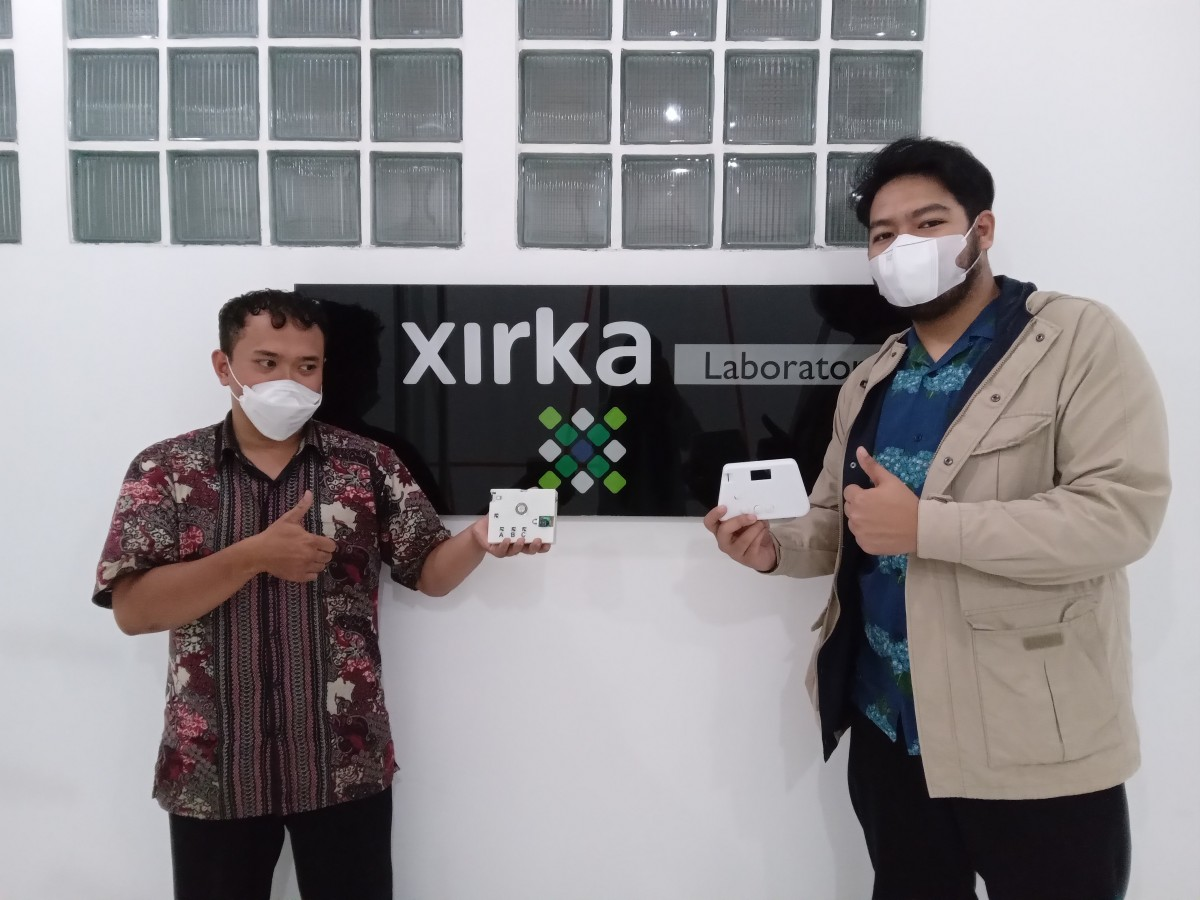
\includegraphics[width=250pt]{images/last_day}
		\end{exampleblock}
	\end{frame}
	
	\section{Kelompok Pekerjaan}
	\begin{frame}
	    \begin{exampleblock}{Kelompok Pekerjaan}
			Lingkup utama pekerjaan yang dilakukan meliputi:
			\begin{itemize}
				\item Assembly 1 unit PCB untuk desain Audiometri P2.
				\item Review Sinyal dan Tone-Generation dari Class-D Audio DAC MAX98357A.
				\item Review sementara desain Audiometri P3.
				\item Upgrade unit packaging untuk Audiometri P2.
			\end{itemize}
	    \end{exampleblock}
	\end{frame}
	
	\section{Assembly PCB}
	\begin{frame}
		\subsection{Tujuan}
		\begin{exampleblock}{Assembly PCB}
			Merakit 1 unit tambahan PCB untuk desain Audiometri P2.
		\end{exampleblock}
	
		\subsection{Hasil}
		\begin{exampleblock}{Assembly PCB}
			Unit tambahan telah terakit
			\begin{center}
				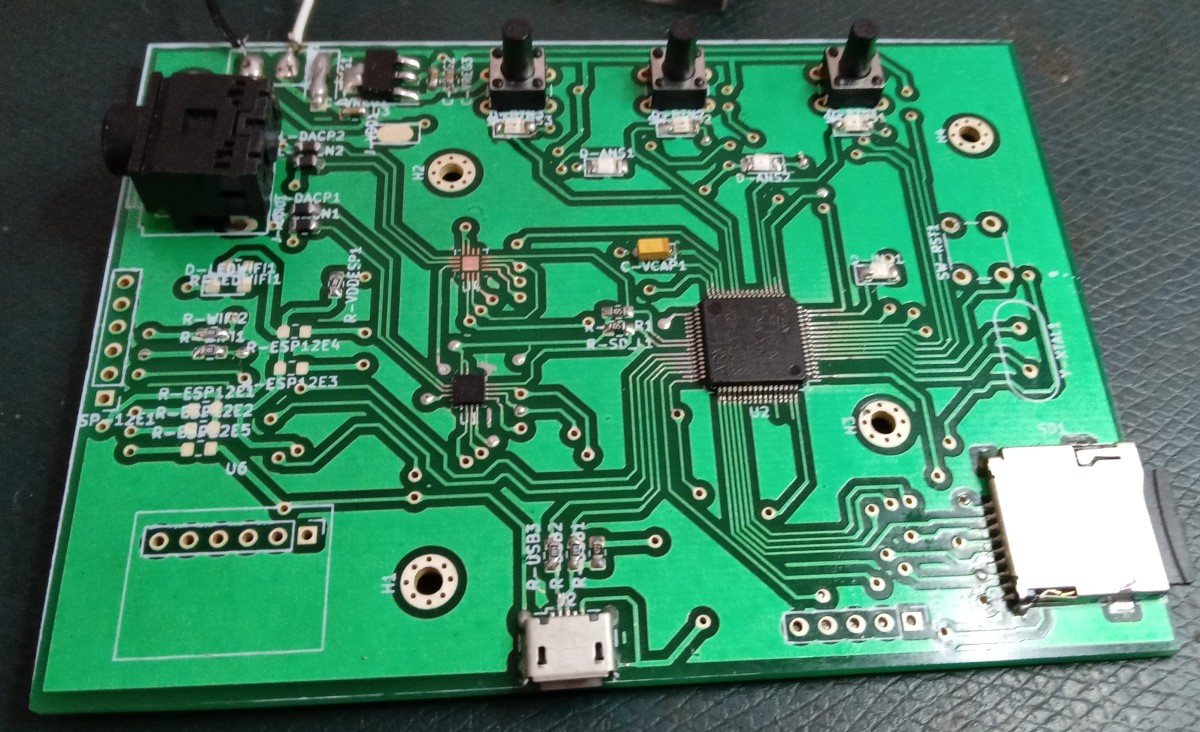
\includegraphics[width=200pt]{images/assembly_hasil}
			\end{center}
		\end{exampleblock}
	\end{frame}

	
	\begin{frame}
		\subsection{Dokumentasi}
		\begin{exampleblock}{Memulai Assembly}
			\begin{center}
				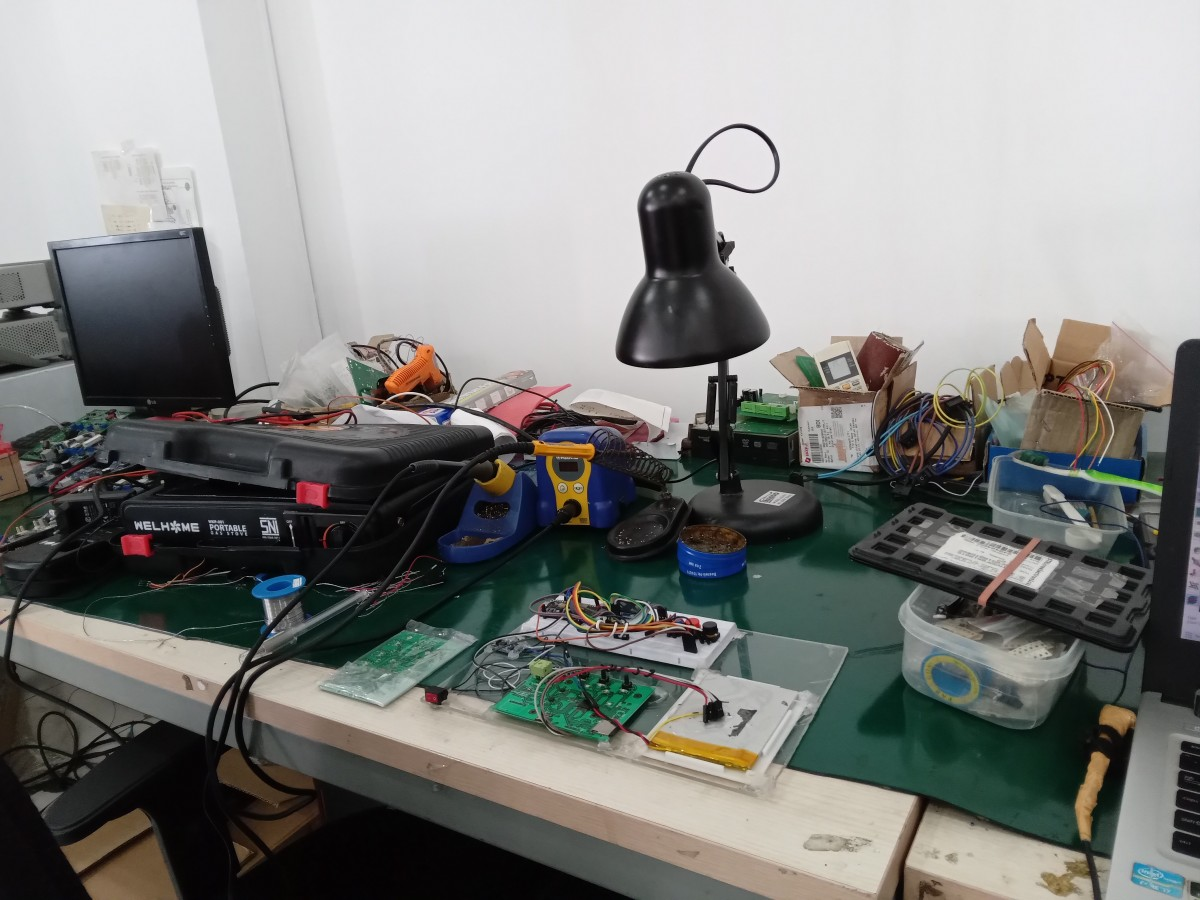
\includegraphics[width=150pt]{images/assembly_unpack}
				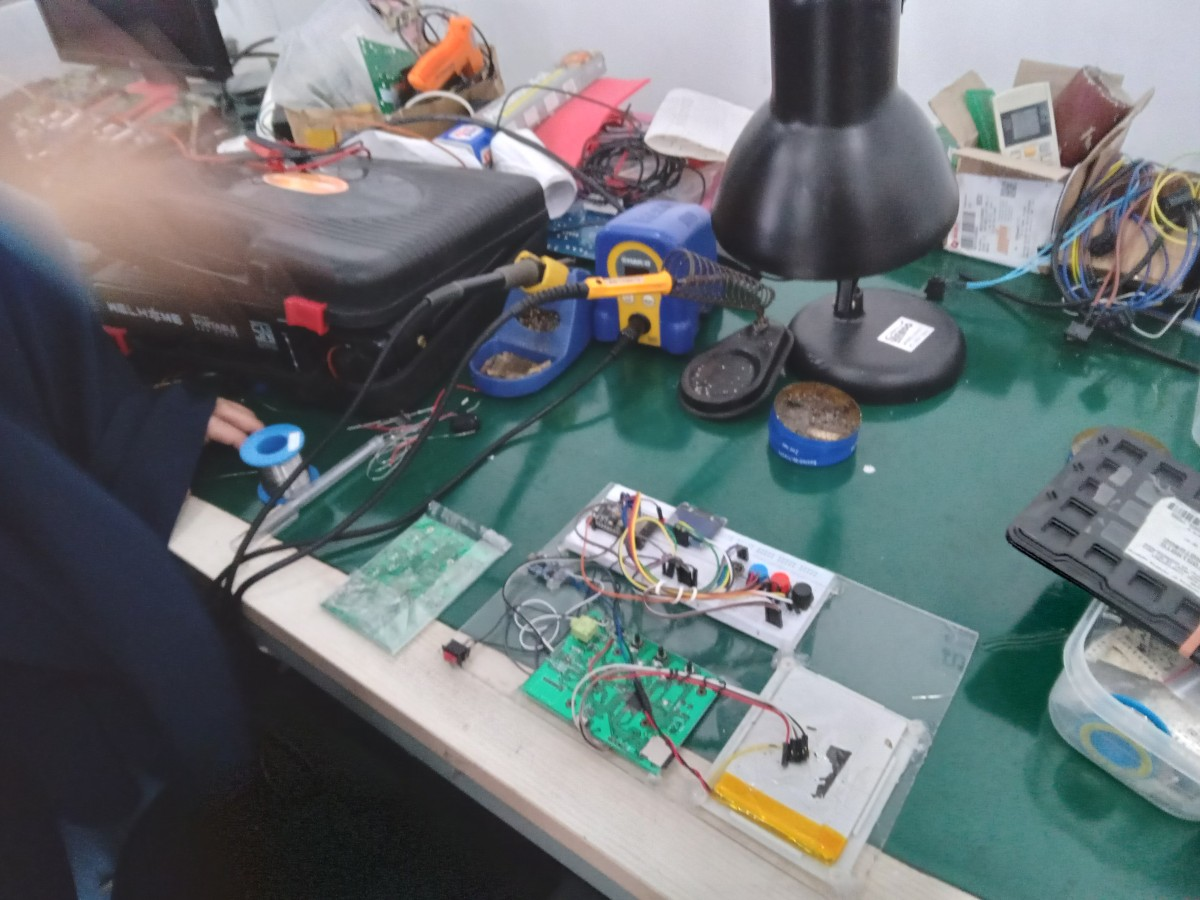
\includegraphics[width=150pt]{images/assembly_start}
			\end{center}
		\end{exampleblock}
	\end{frame}

	\begin{frame}
		\begin{exampleblock}{Proses Soldering Manual}
			\begin{center}
				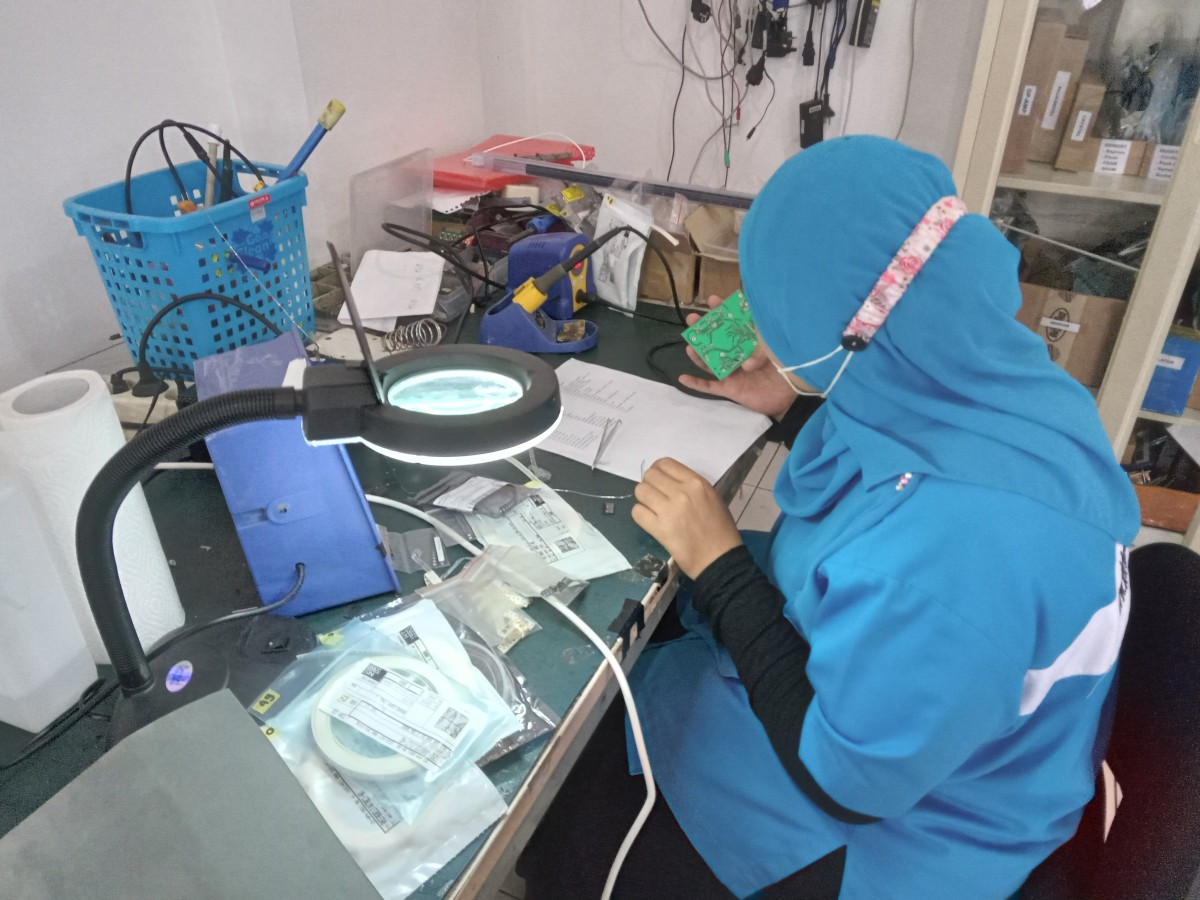
\includegraphics[width=200pt]{images/assembly_manual}
			\end{center}
		\end{exampleblock}
	\end{frame}

	\section{Review Class-D Audio DAC}
	
	\begin{frame}
		\subsection{Tujuan}
		\begin{exampleblock}{Review Class-D AudioDAC}
			Audio Digital to Analog chip yang digunakan adalah seri MAX98357A yang merupakan audio amplifier kelas D.
			Ditemukan frekuensi lebih dari satu frekuensi setiap proses \textit{tone generation} yang muncul saat diuji dengan Audio Capture.
			Perangkat Audio Capture yang digunakan adalah MiniDSP E.A.R.S melalui software DSSF3 buatan Yoshimasha.
		\end{exampleblock}
	
		\begin{exampleblock}{MiniDSP EARS}
			\begin{center}
				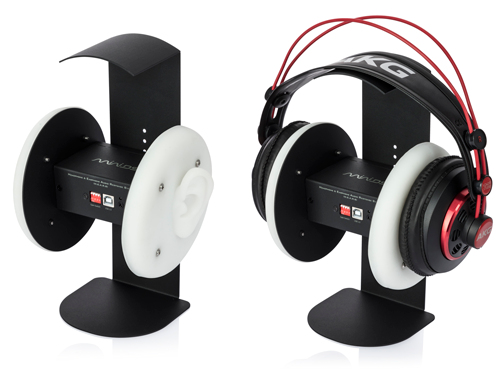
\includegraphics[width=150pt]{images/ears}
			\end{center}
		\end{exampleblock}
	\end{frame}

	\begin{frame}
		\subsection{High Frequency Noise}
		\begin{exampleblock}{Perbandingan penuh dan teratenuasi}
			\begin{center}
				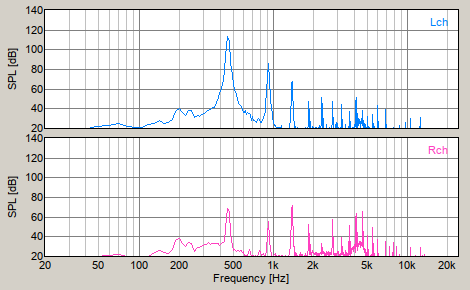
\includegraphics[width=200pt]{images/notattenuated}
				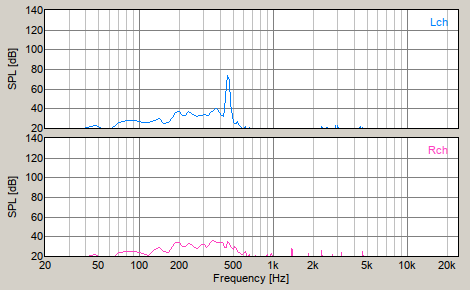
\includegraphics[width=200pt]{images/attenuated}
			\end{center}
		\end{exampleblock}
	\end{frame}
	
	\begin{frame}[fragile]
		\subsection{Signal Generation Code}
		\begin{exampleblock}{Perbaikan Programming}
			Dilakukan perbaikan \textit{programming} terkait metode \textit{tone generation}
		\end{exampleblock}
	
		\begin{exampleblock}{Diff code}
			\begin{minted}[frame=lines,framesep=2mm,baselinestretch=1.2,bgcolor=LightGray,fontsize=\tiny,linenos]{diff}
-static uint16_t i2s_tx_buf[TOTAL_BUFF_SIZE];
+int16_t i2s_tx_buf[TOTAL_BUFF_SIZE];

uint16_t i;
uint16_t buffsize;
double ysin;

for(i=0;i<buffsize;i++){
	ysin = DEFAULT_ATTEN*ampl*32767*sin(2*3.141592653589793*((double)i/(double)buffsize));
	
-	if(ysin >= 0){
-		i2s_tx_buf[i]=ysin;
-	}
-	if(ysin < 0){
-		i2s_tx_buf[i]=ysin+65535;
-	}
+ 	i2s_tx_buf[i] = ysin;
}
			\end{minted}
		\end{exampleblock}
	\end{frame}

	\begin{frame}
		\begin{exampleblock}{Model sinus sebelum/sesudah perbaikan}
			\begin{center}
				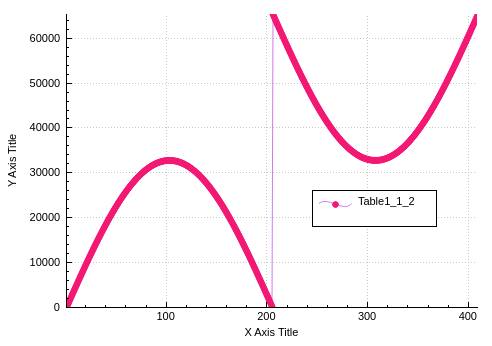
\includegraphics[width=165pt]{images/weird_sine}
				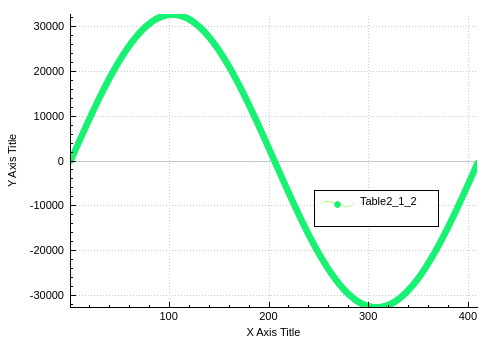
\includegraphics[width=165pt]{images/normal_sine}
			\end{center}
		\end{exampleblock}
	\end{frame}

	\begin{frame}
		\subsection{Clipping Limitation}
		\begin{exampleblock}{pembacaan output penuh/atenuasi (OSC: Keysight MSO-X 2002A)}
			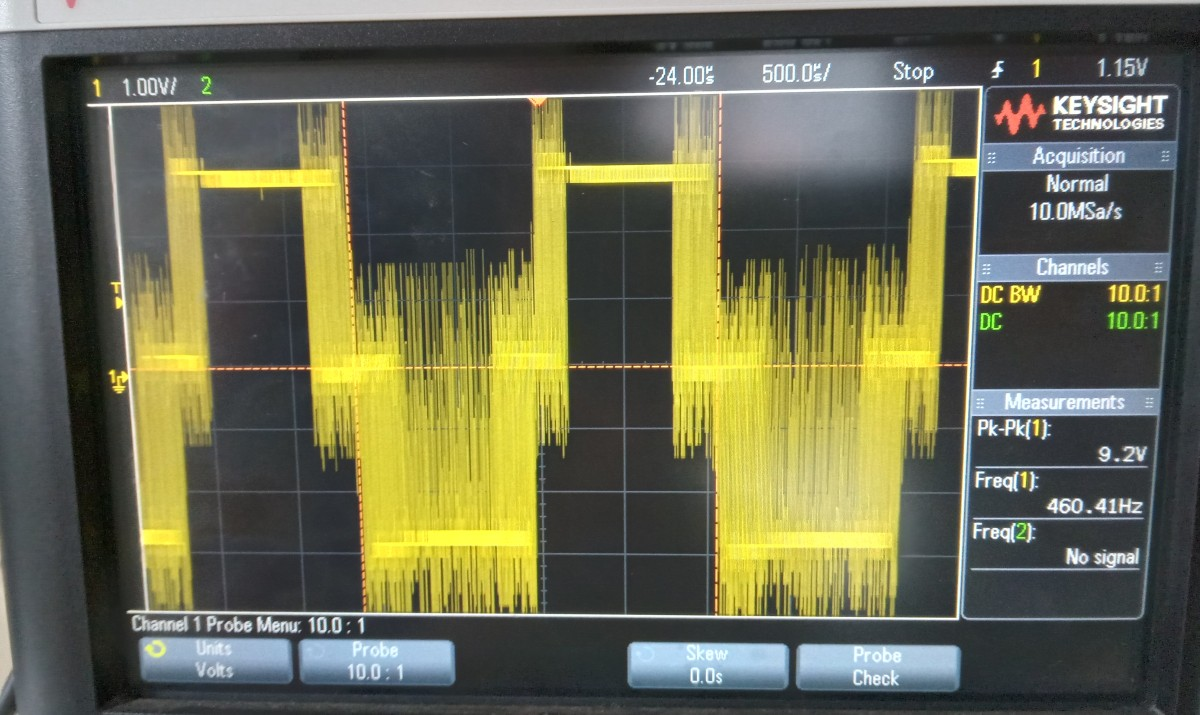
\includegraphics[width=165pt]{images/sinefull_osc}
			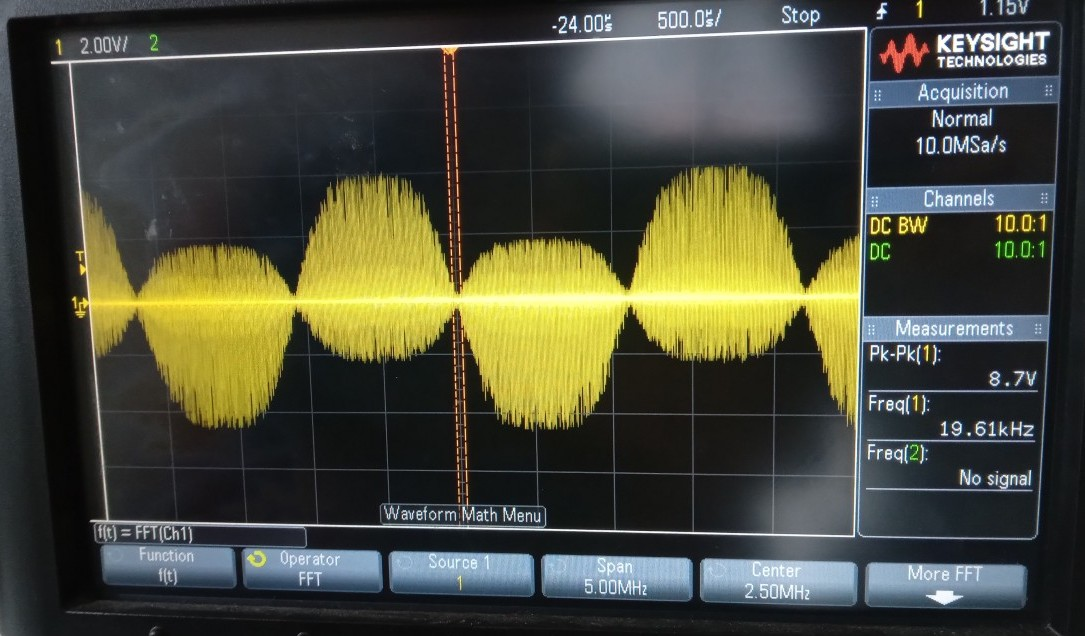
\includegraphics[width=165pt]{images/sine_osc}
		\end{exampleblock}
		
		\begin{exampleblock}{prinsip Fourier series pada square wave}
			\centering
			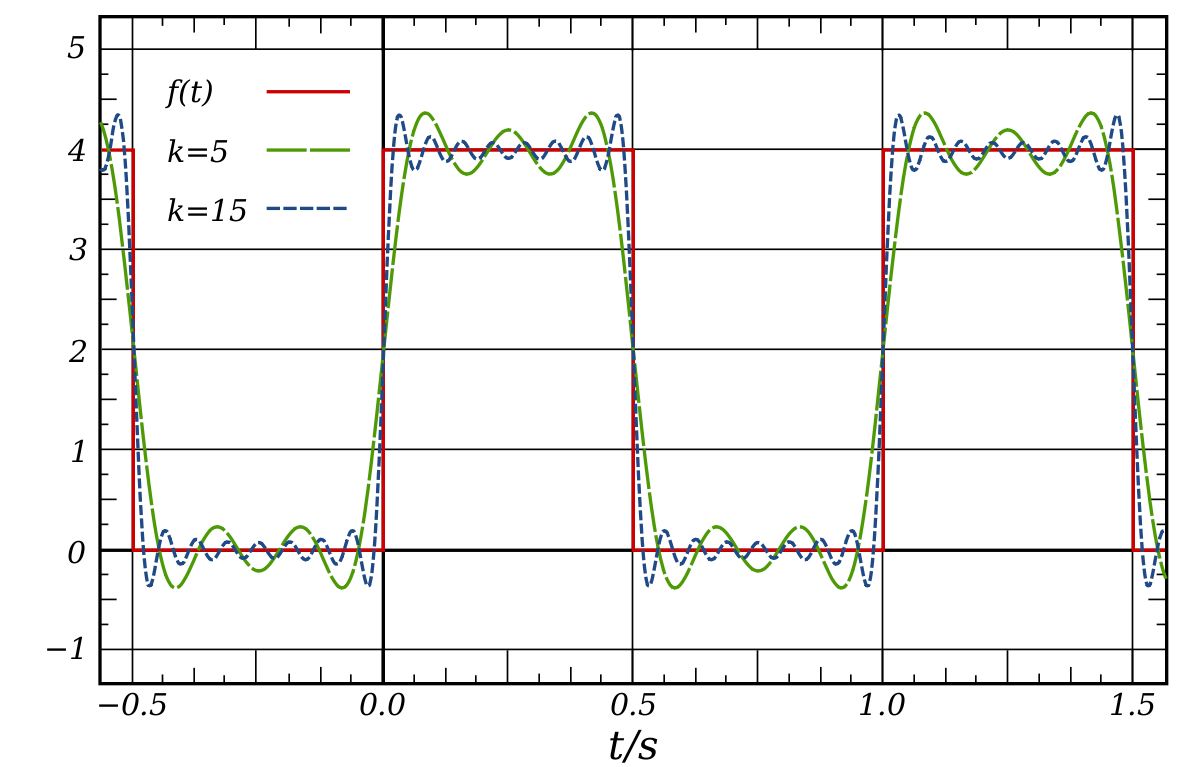
\includegraphics[width=150pt]{images/square_wave_fourier}
		\end{exampleblock}
	\end{frame}
	
	\begin{frame}
		\subsection{Compare to Signal Generator}
		\begin{exampleblock}{Tes sine-wave  (OSC: Siglent SDS 1072CML)}
			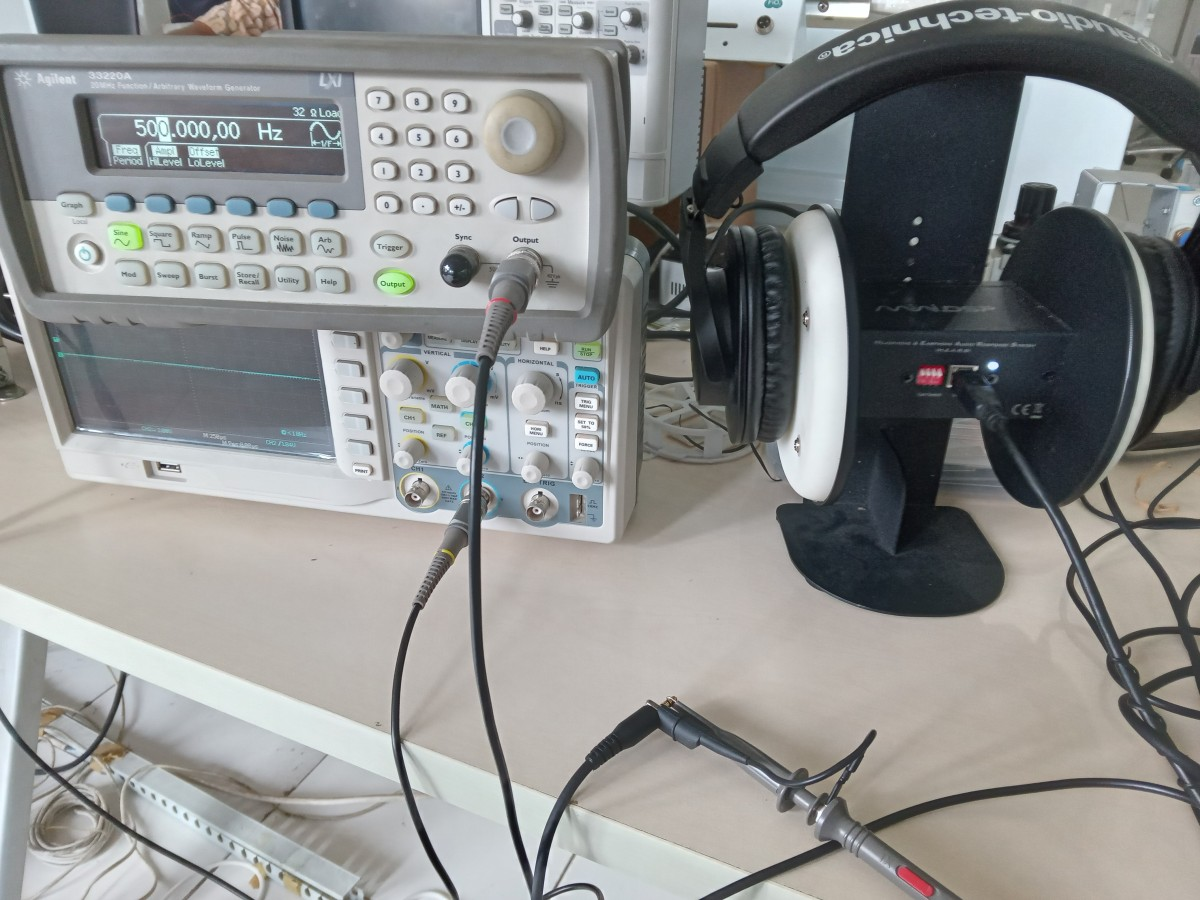
\includegraphics[width=150pt]{images/sine_sig_test}
			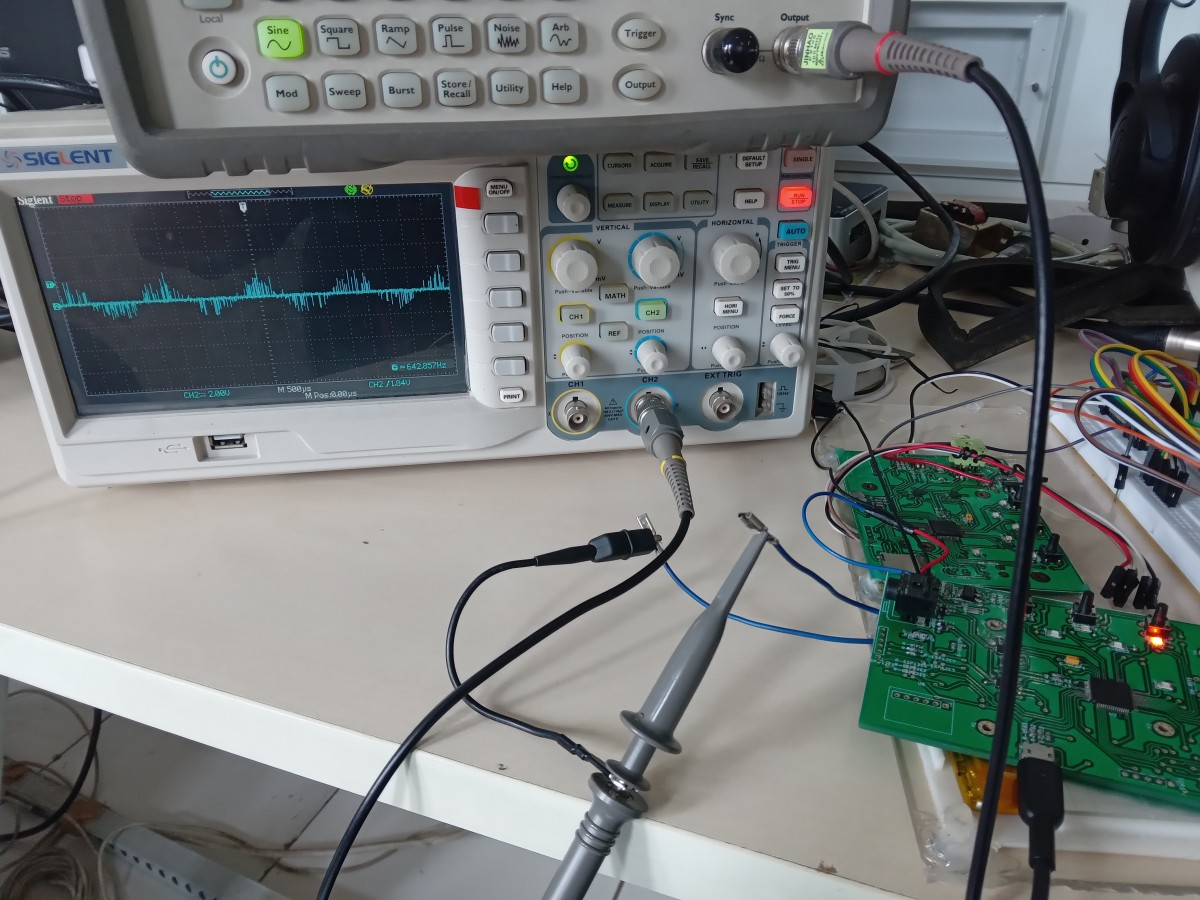
\includegraphics[width=150pt]{images/sine_sig_test_dac}
		\end{exampleblock}
	
		\begin{exampleblock}{perbandingan signal generator dan class-D Audio DAC}
			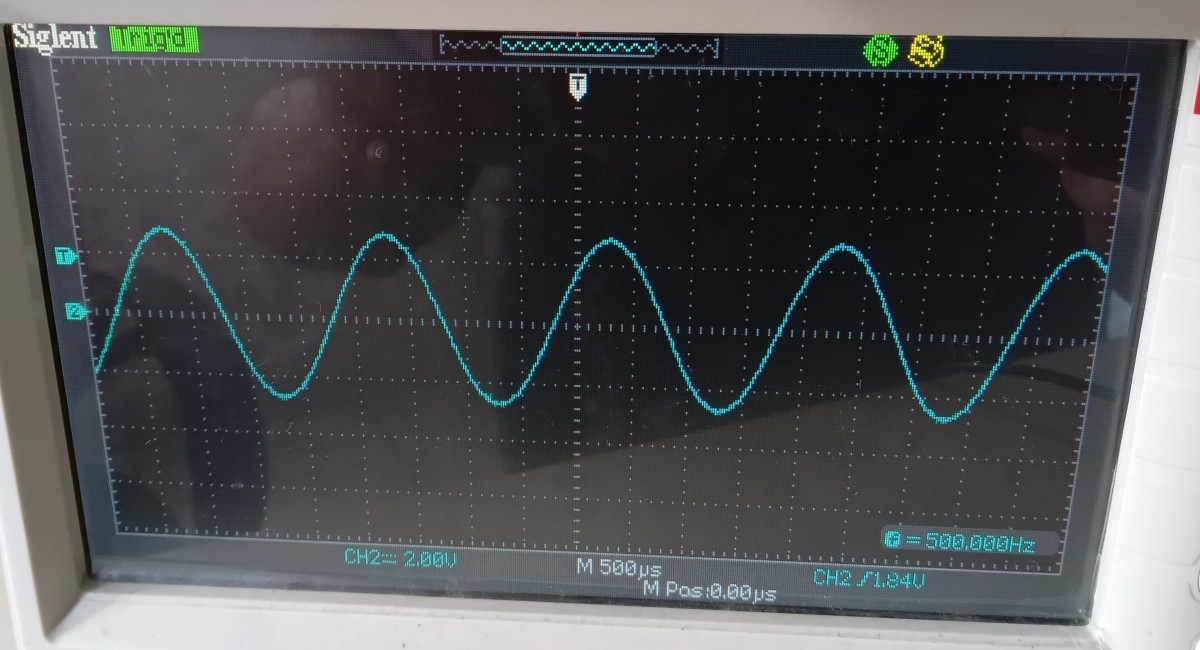
\includegraphics[width=165pt]{images/sine_sig_gen}
			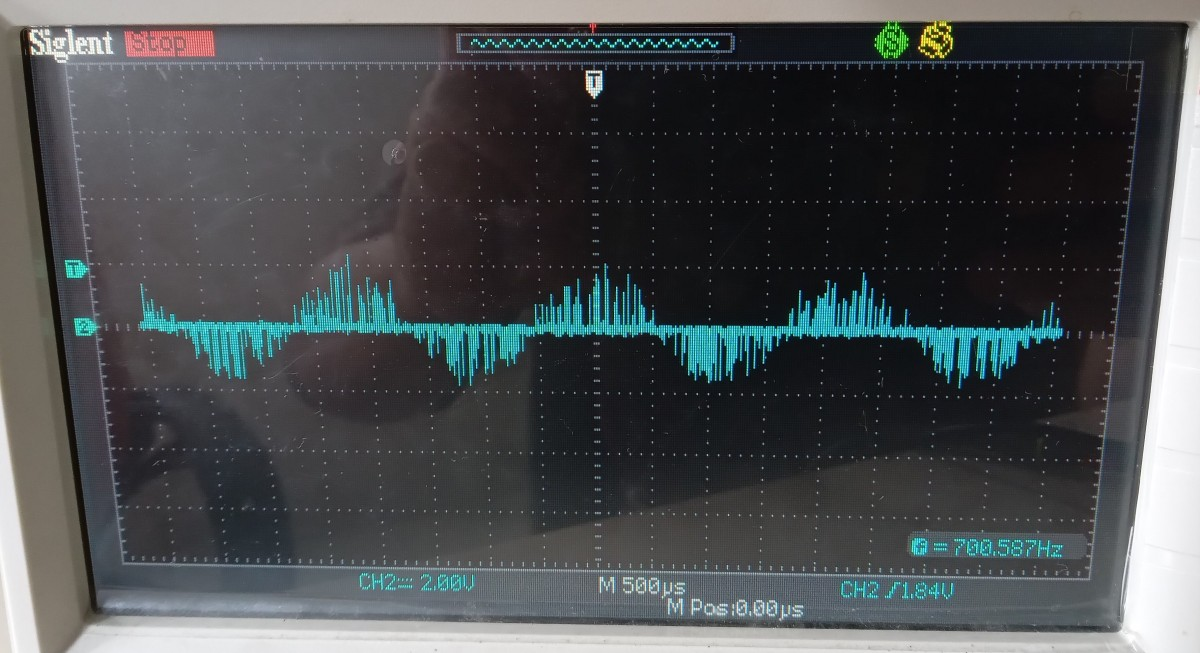
\includegraphics[width=165pt]{images/sine_sig_dac}
		\end{exampleblock}
	\end{frame}
	
	\section {Review Sementara Desain P3}
	
	\begin{frame}
		\begin{exampleblock}{Progress sementara desain P3}
			Berikut progres diagram dasar sistem untuk pengembangan prototype P3 yang di-\textit{draft} di software Altium Designer.
			Terbagi dalam dua grup:
			\begin{itemize}
				\item Diagram Power
				\item Diagram Sinyal
			\end{itemize}
		\end{exampleblock}
	\end{frame}

	\begin{frame}
		\subsection{Diagram Power}
		\begin{exampleblock}{Diagram Power}
			\centering
			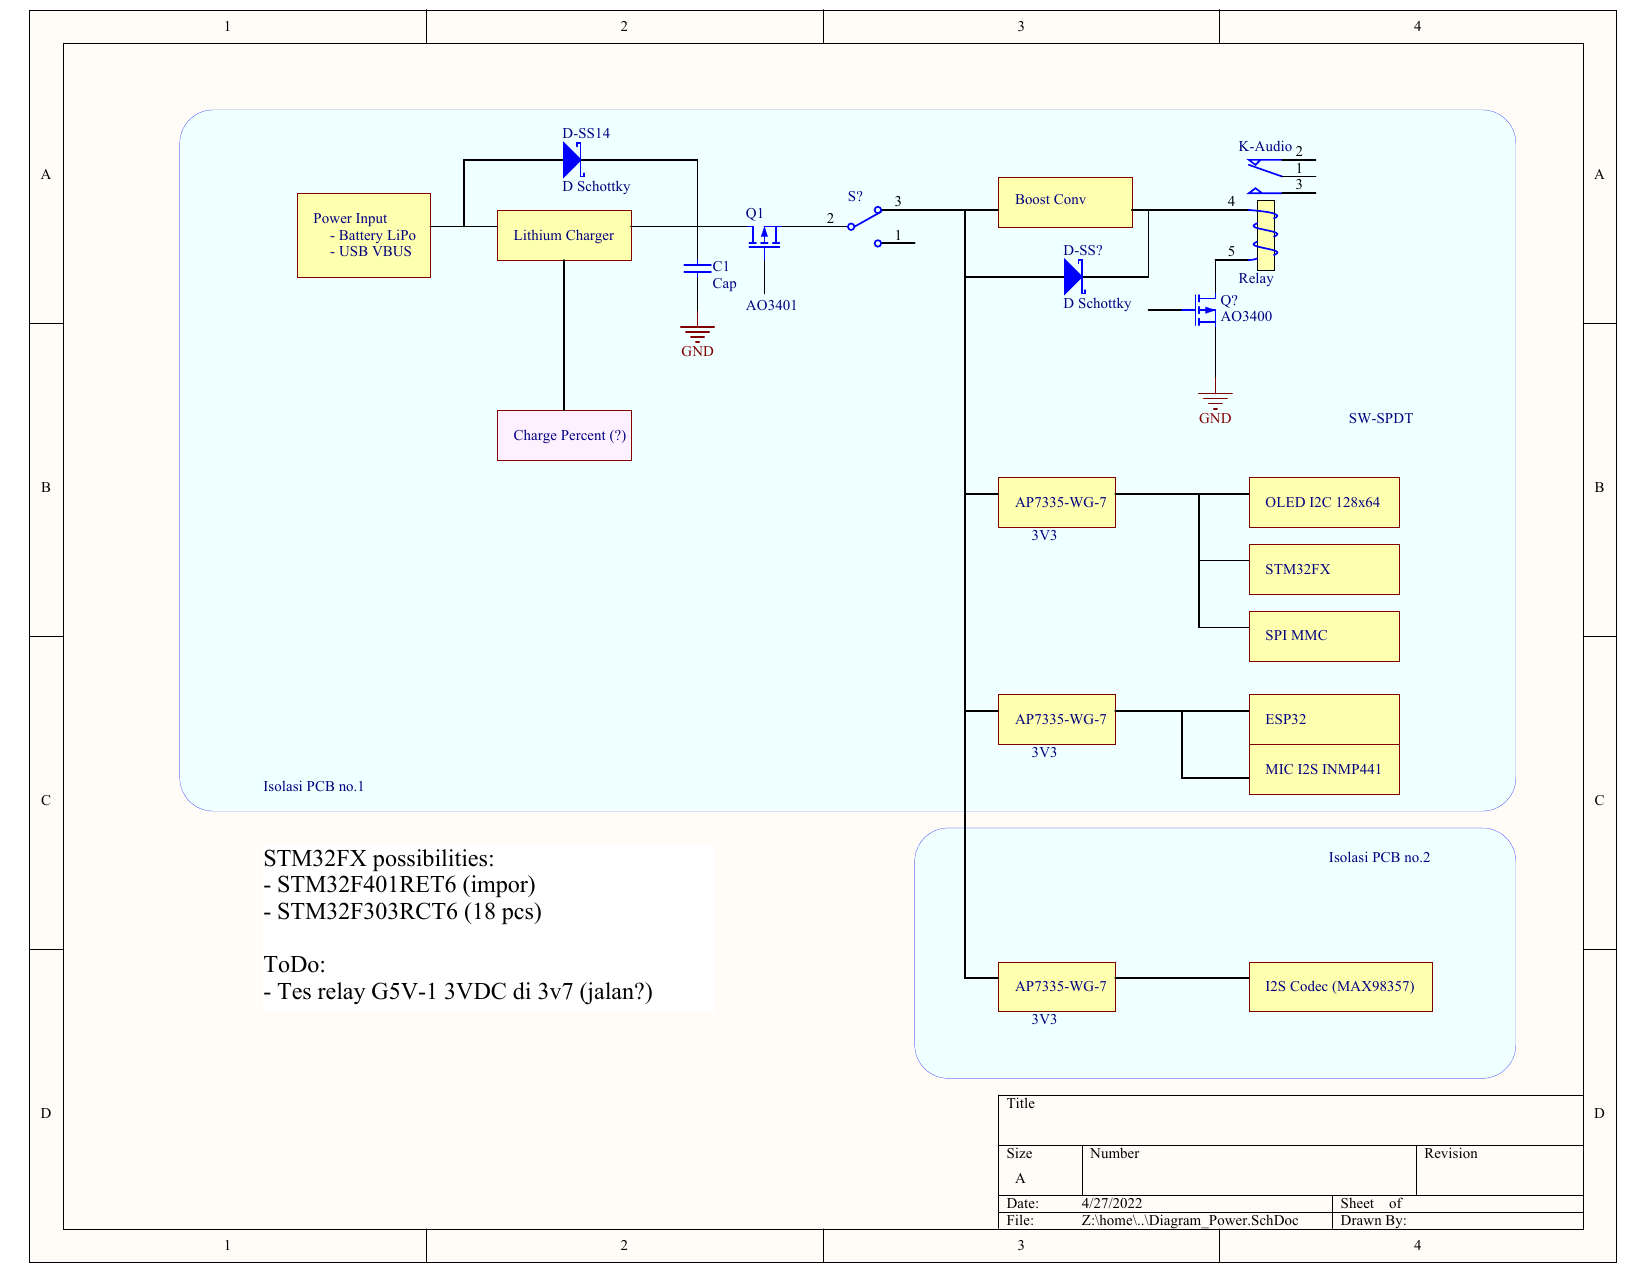
\includegraphics[width=300pt]{images/diagram_power}
		\end{exampleblock}
	\end{frame}

	\begin{frame}
		\subsection{Diagram Signal}
		\begin{exampleblock}{Diagram Signal}
			\centering
			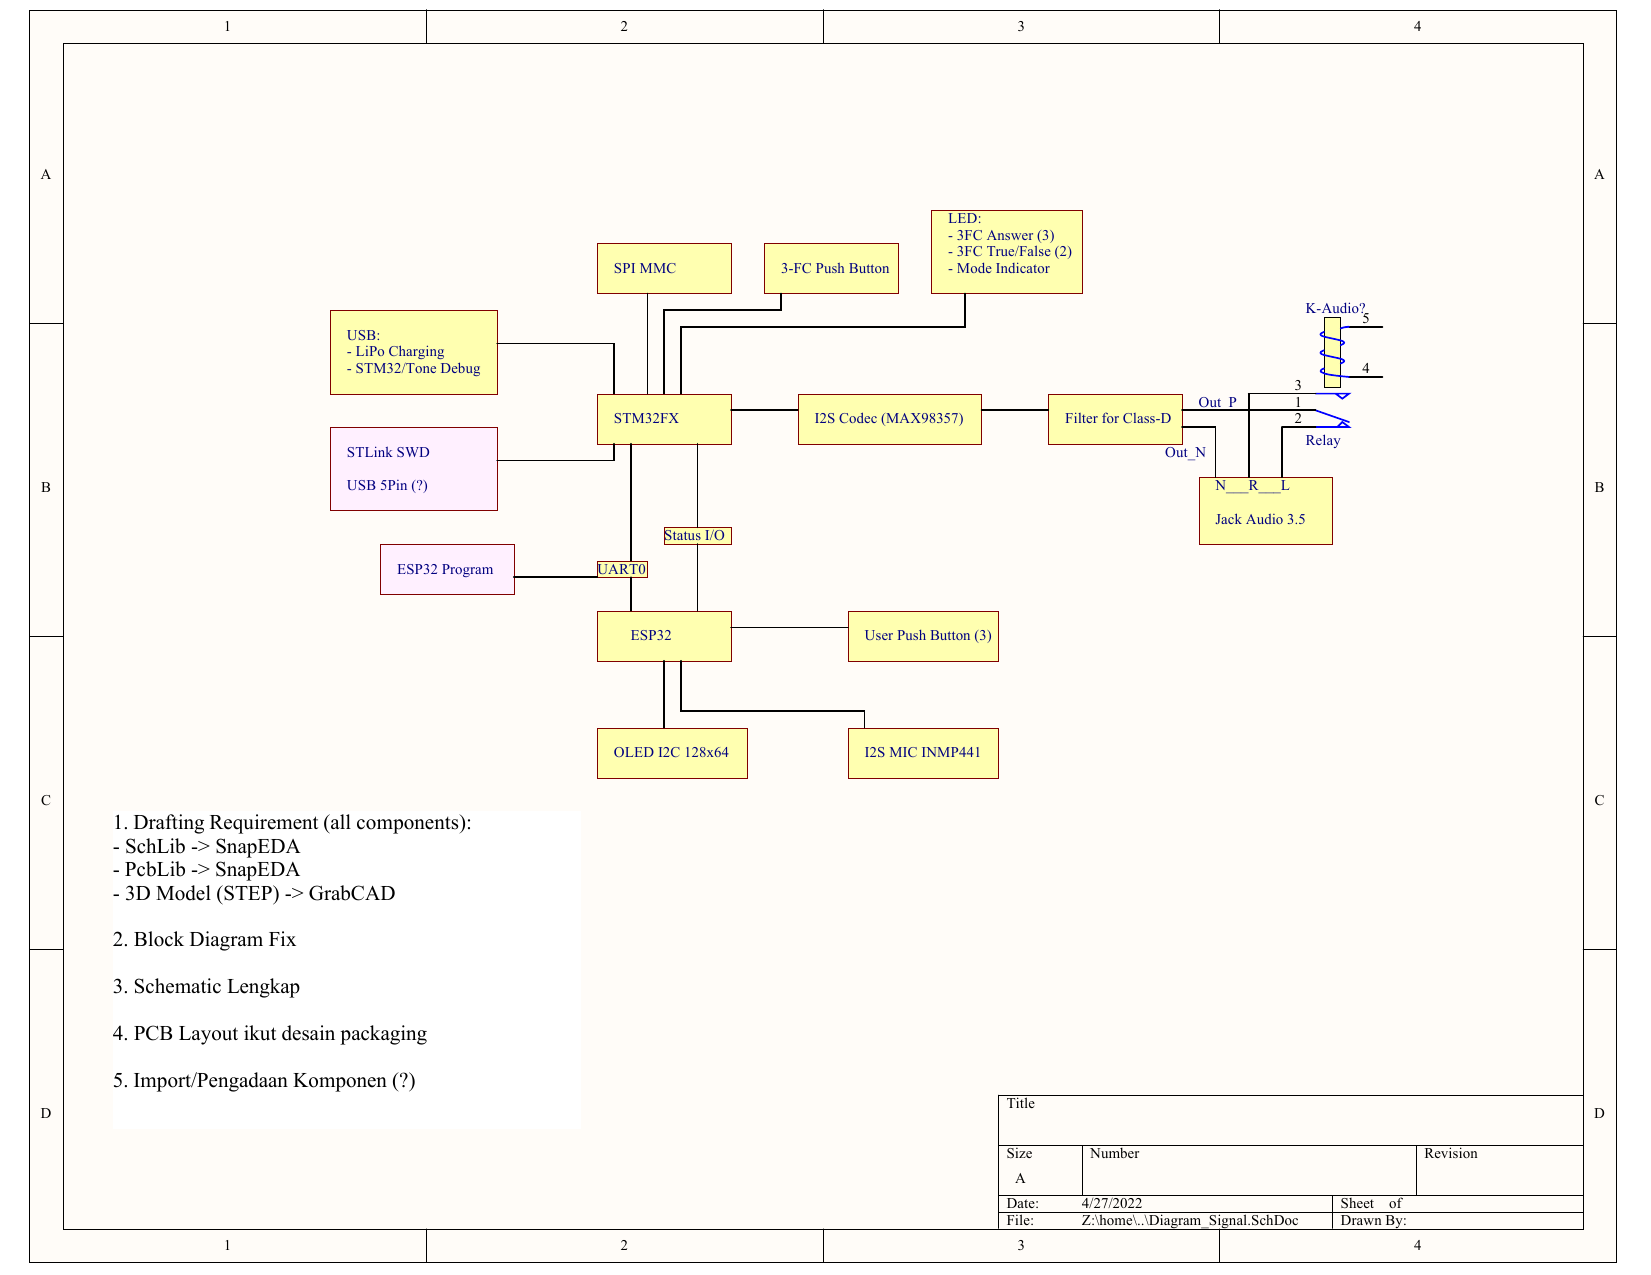
\includegraphics[width=300pt]{images/diagram_signal}
		\end{exampleblock}
	\end{frame}
	
	\section{Upgrade Packaging P2}
	
	\begin{frame}
		\subsection{Tujuan}
		\begin{exampleblock}{Upgrade Packaging}
			Telah dilakukan upgrade desain packaging dan merakit 3D-print desain tersebut untuk prototype P2 sehingga pengunaan menjadi lebih nyaman.
		\end{exampleblock}
	
		\subsection{Hasil}
		\begin{exampleblock}{Perbandingan packaging lama/baru}
			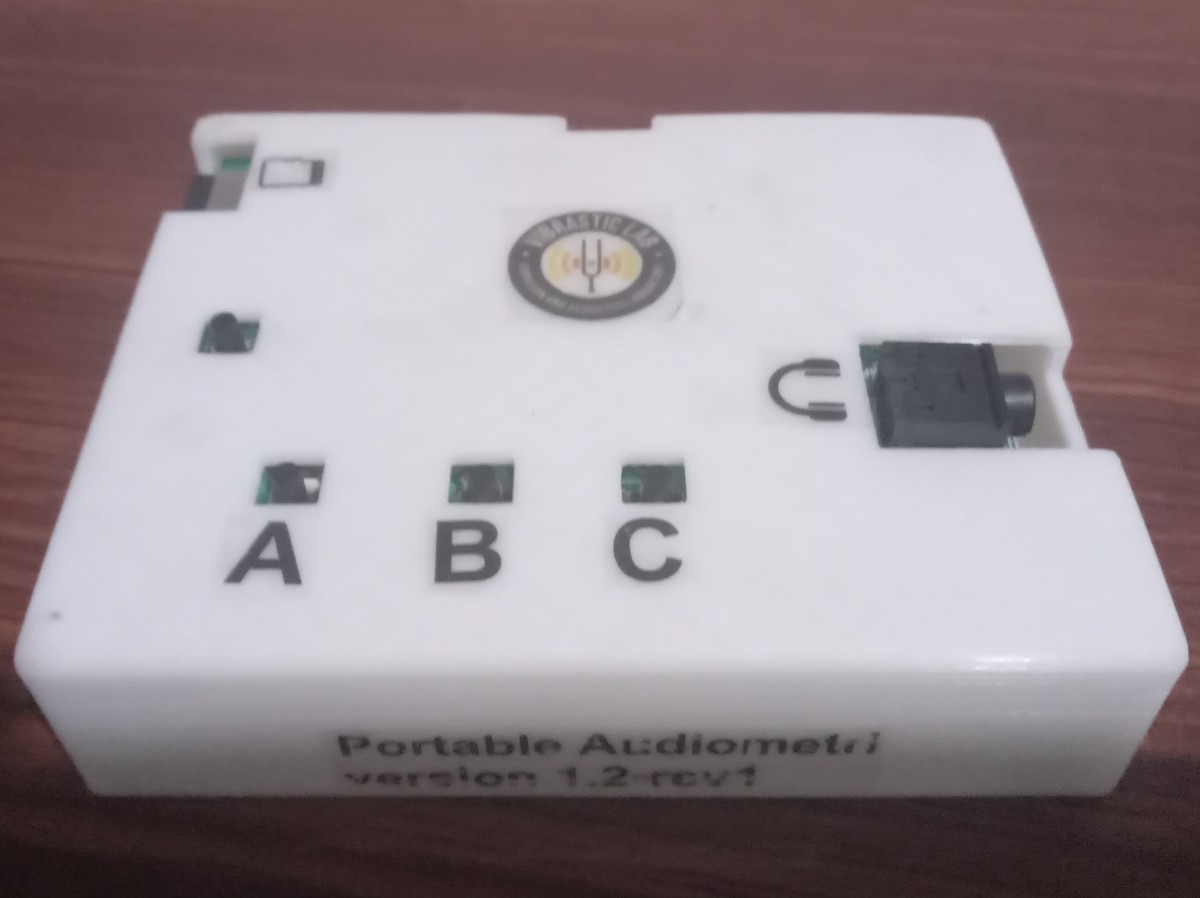
\includegraphics[width=165pt]{images/pack_lama}
			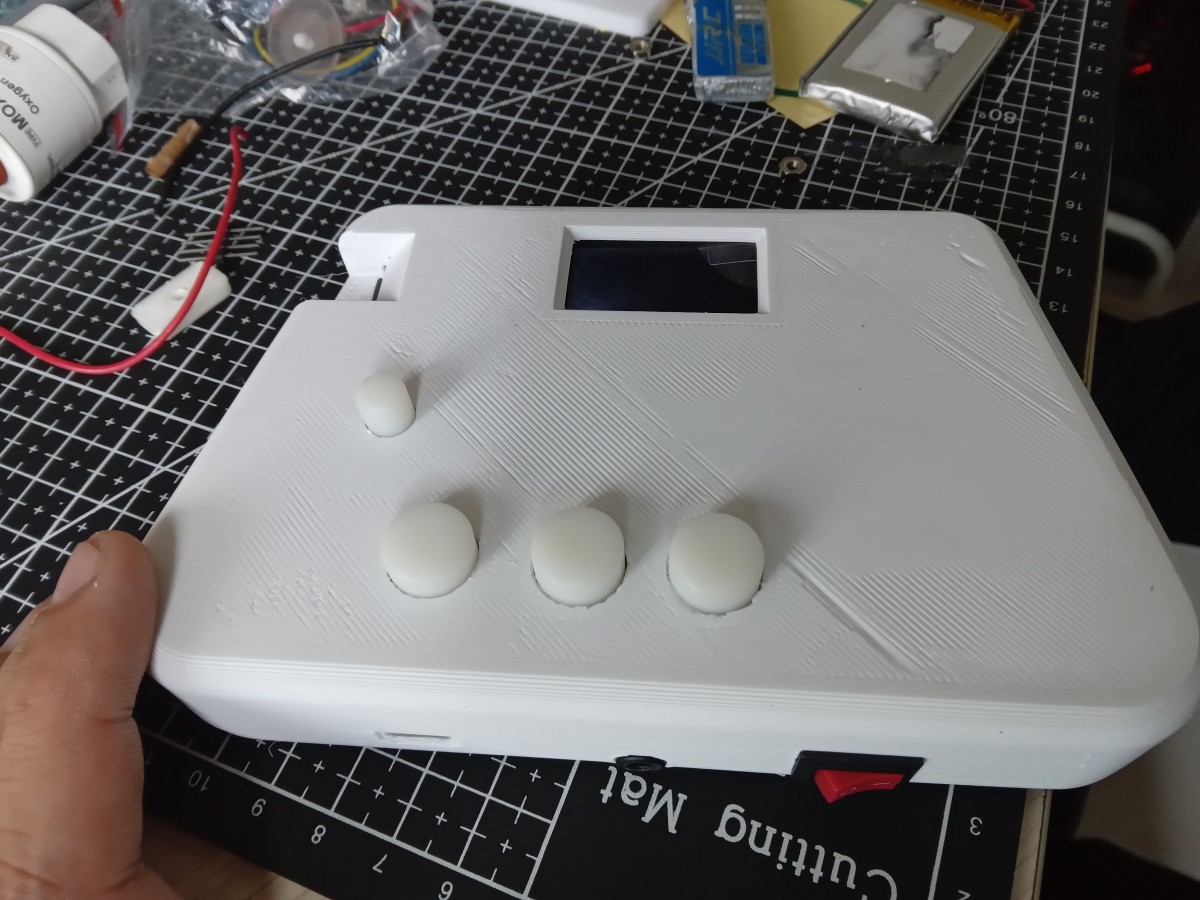
\includegraphics[width=165pt]{images/pack_jadi}
		\end{exampleblock}
	\end{frame}

	\begin{frame}
		\subsection{Dokumentasi}
		\begin{exampleblock}{Dokumentasi}
			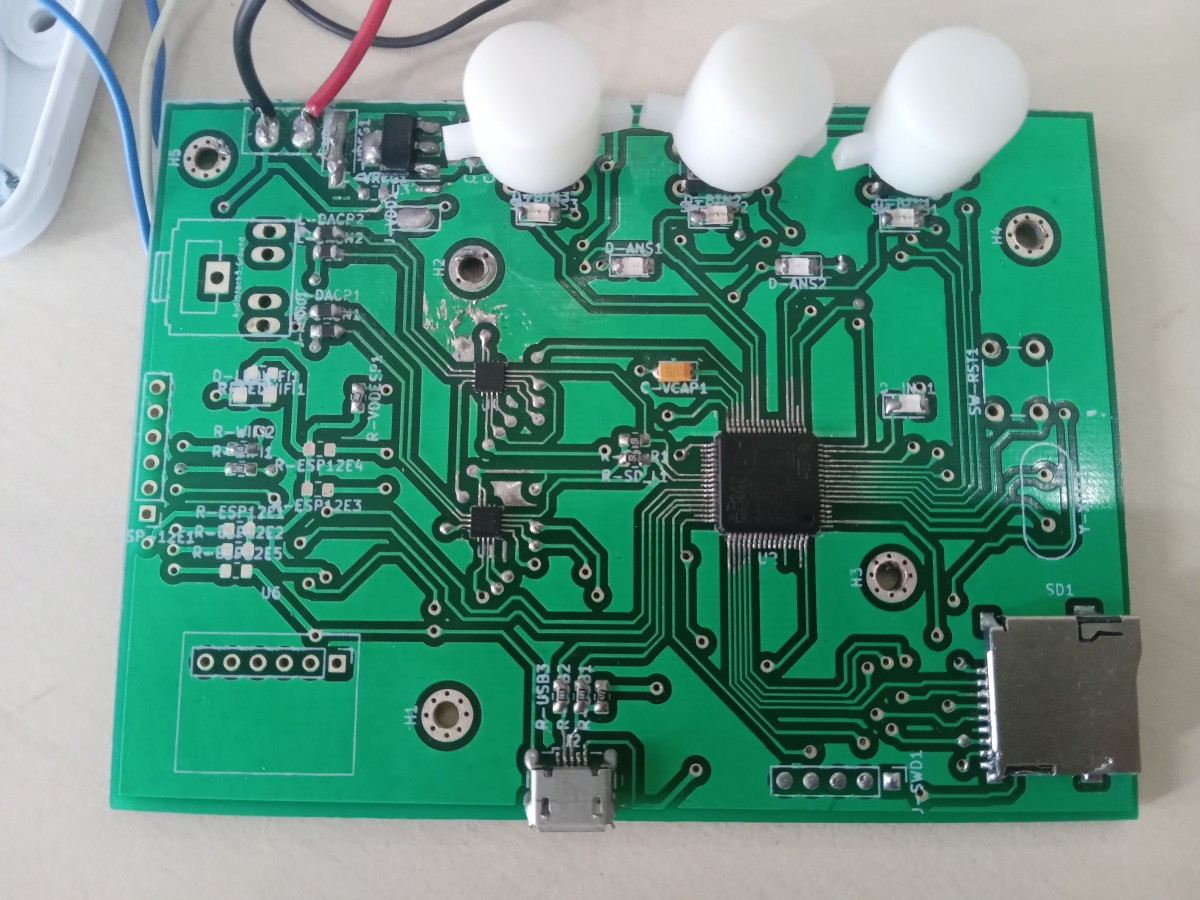
\includegraphics[width=165pt]{images/pack_open0}
			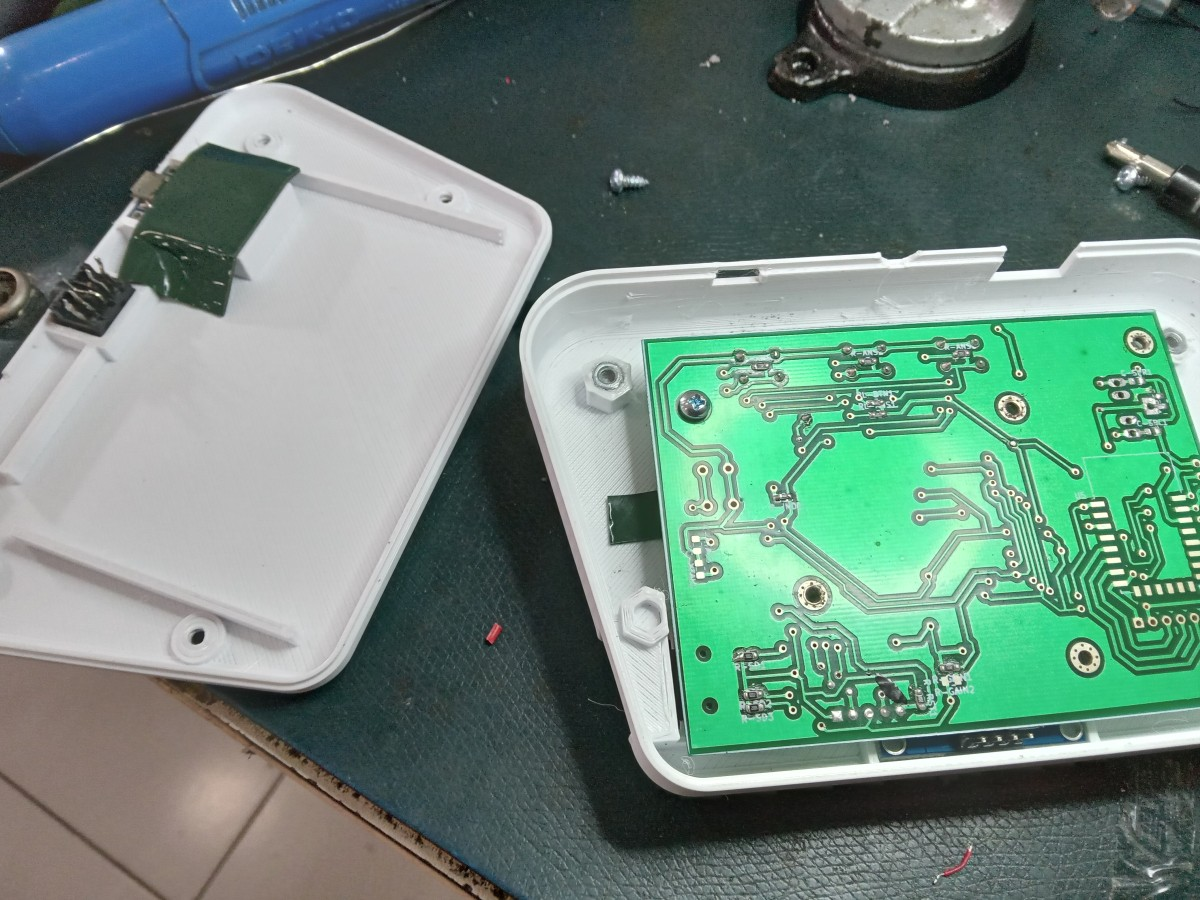
\includegraphics[width=165pt]{images/pack_open1}
		\end{exampleblock}
	
		\begin{exampleblock}{Modifikasi PCB}
			Beberapa modifikasi circuit P2:
			\begin{itemize}
				\item Ukuran/luasan fisik battery harus lebih kecil
				\item Jack Audio 3.5mm di-\textit{wiring} di luar PCB
			\end{itemize}
		\end{exampleblock}
	\end{frame}
	
	\section{Pengadaan Inventaris}
	
	\subsection{Examples}
	\begin{frame}
		\begin{exampleblock}{Pengadaan/pembaharuan peralatan}
			Berikut beberapa contoh peralatan yang dapat dilakukan pengadaan/pembaharuan.
		\end{exampleblock}
	
		\begin{exampleblock}{Solder tipe tip Knife (K-series) plus regulator}
			\centering
			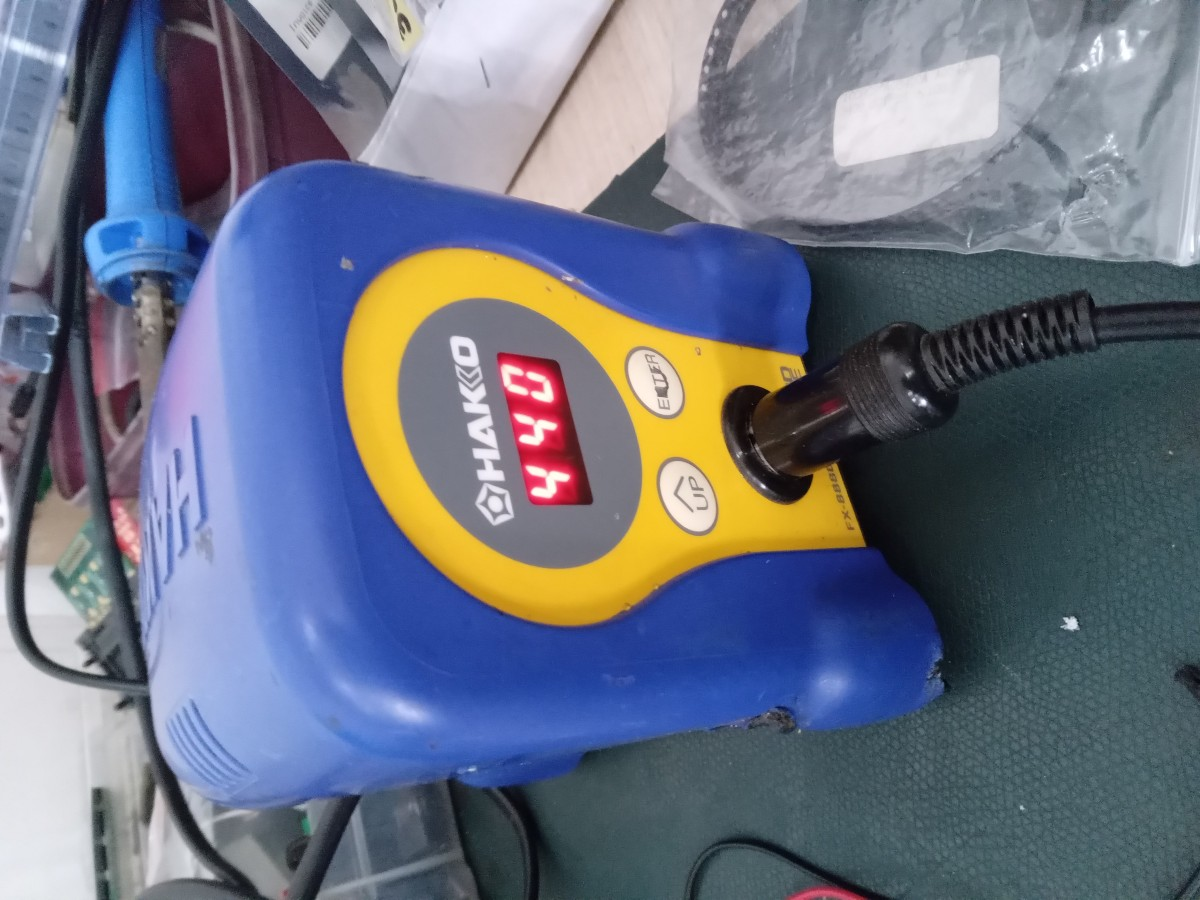
\includegraphics[width=165pt,angle=-90,origin=c]{images/solder0}
			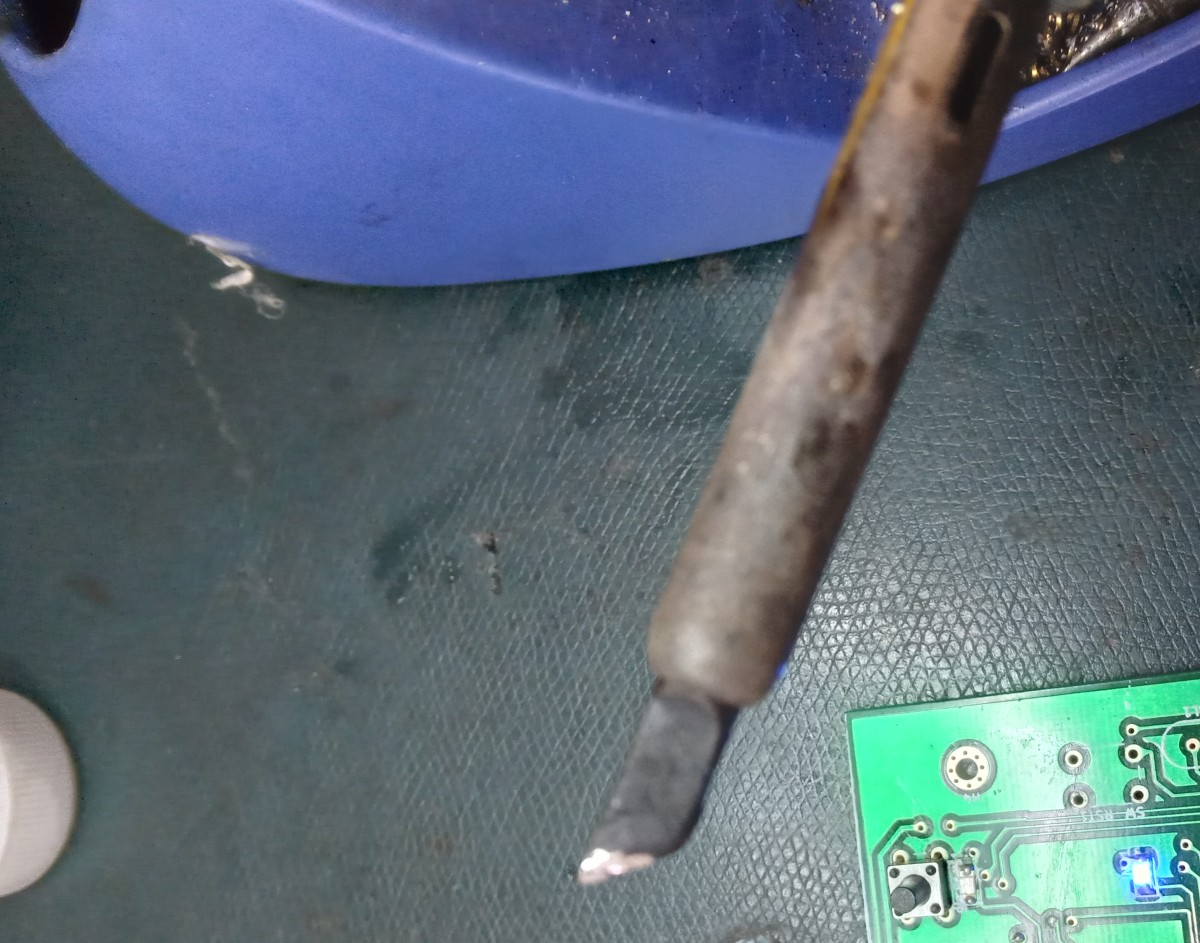
\includegraphics[width=165pt,angle=-90,origin=c]{images/solder1}
		\end{exampleblock}
	\end{frame}

	\begin{frame}
		\begin{exampleblock}{Timah wire dan LotFet (Tidak perlu timah Mechanical)}
			\centering
			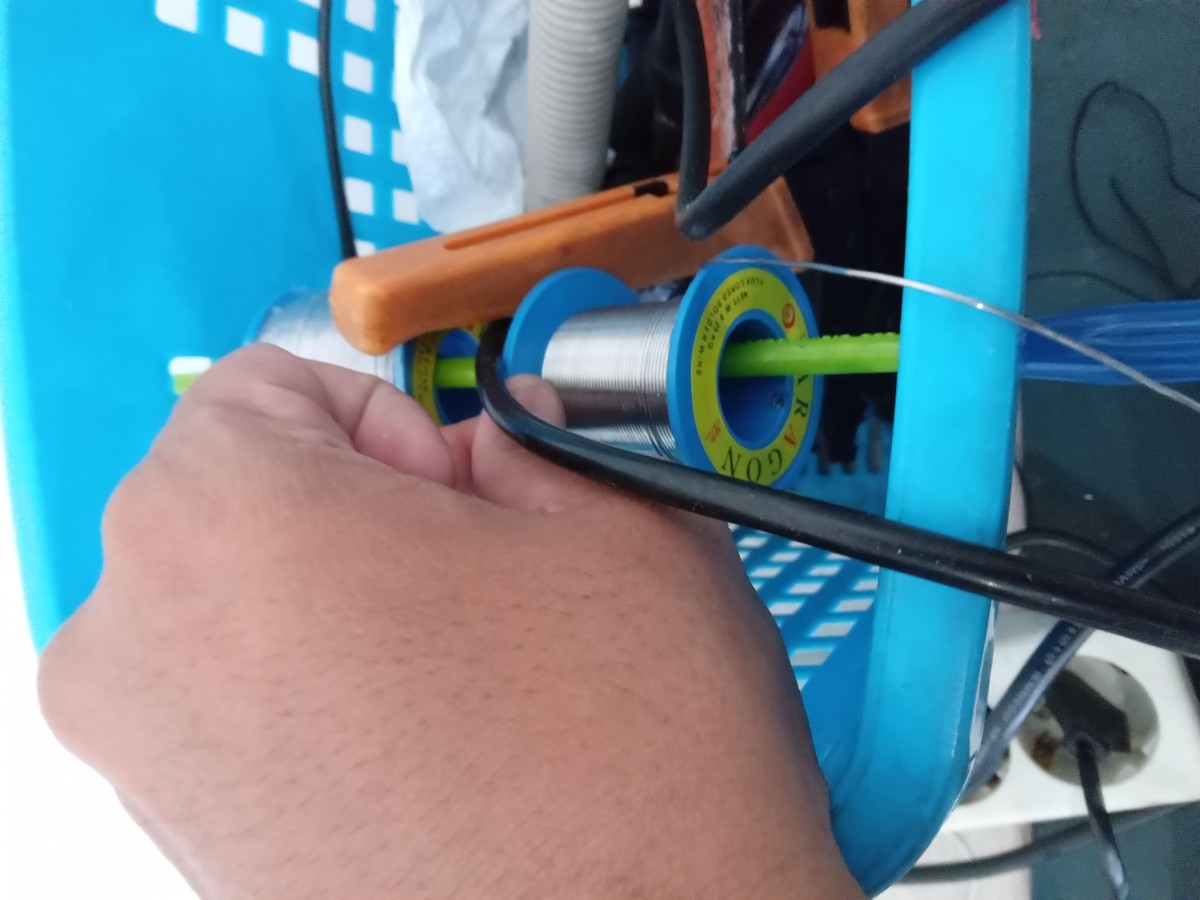
\includegraphics[width=100pt,angle=-90,origin=c]{images/timah}
			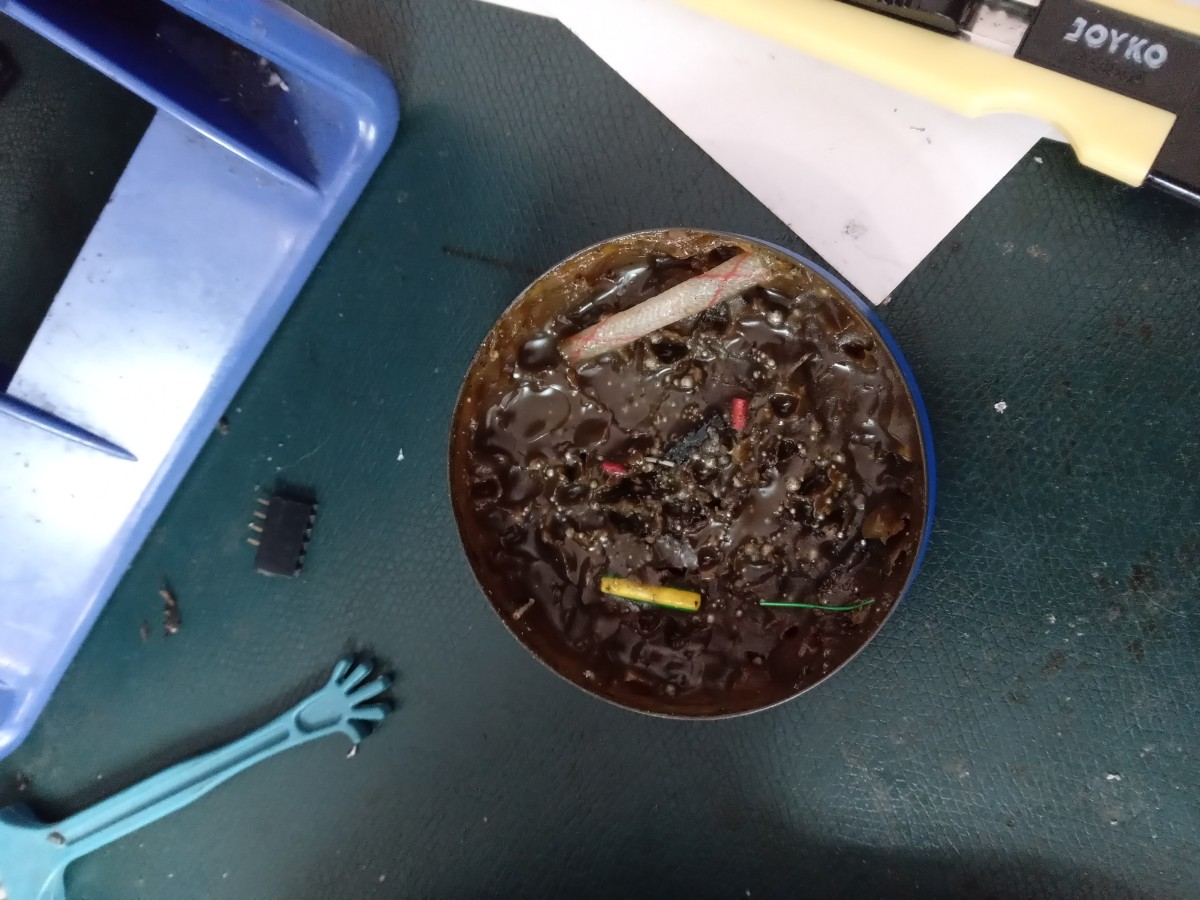
\includegraphics[width=100pt,angle=-90,origin=c]{images/lotfet}
		\end{exampleblock}
		
		\begin{exampleblock}{PCB Cleaner (isopropyl alcohol dan quick-absorb tissue)}
			\centering
			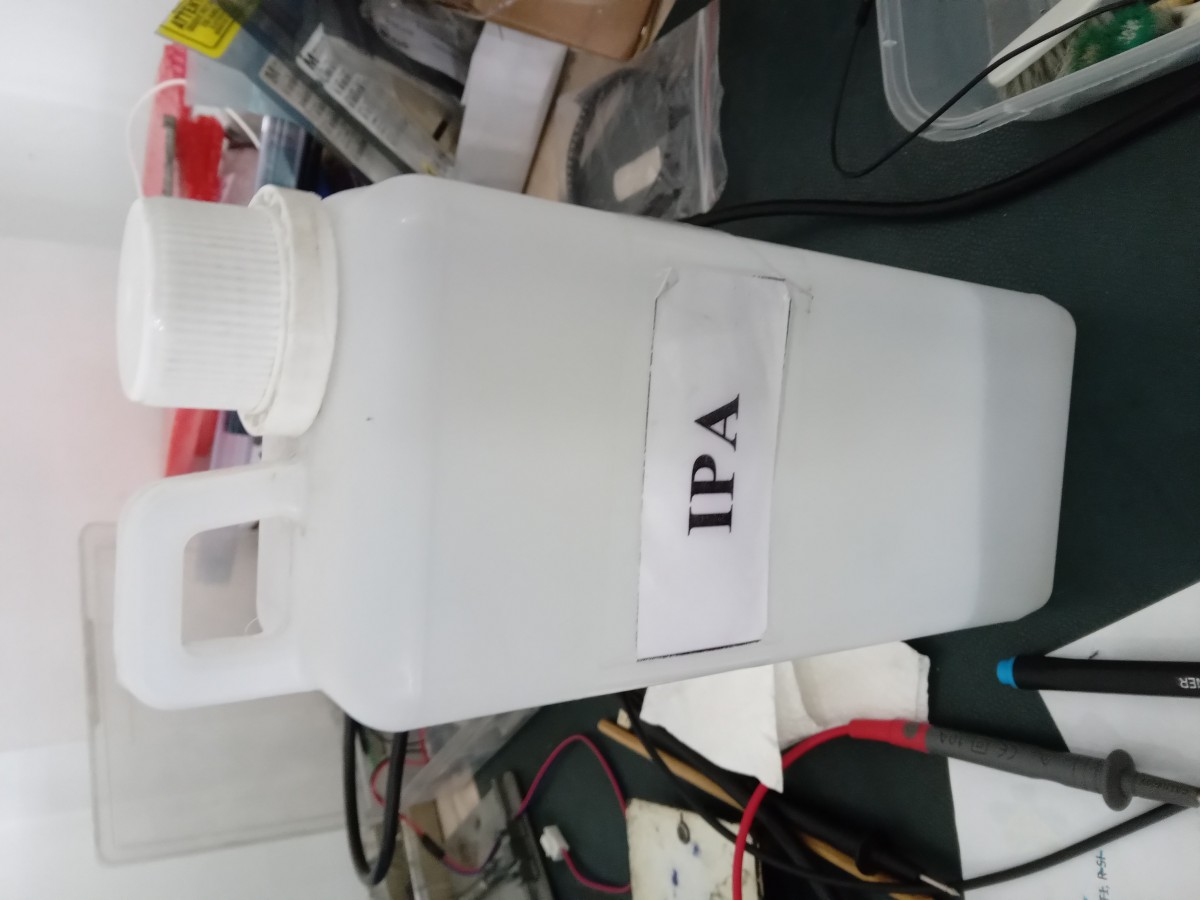
\includegraphics[width=100pt,angle=-90,origin=c]{images/pcbclean0}
			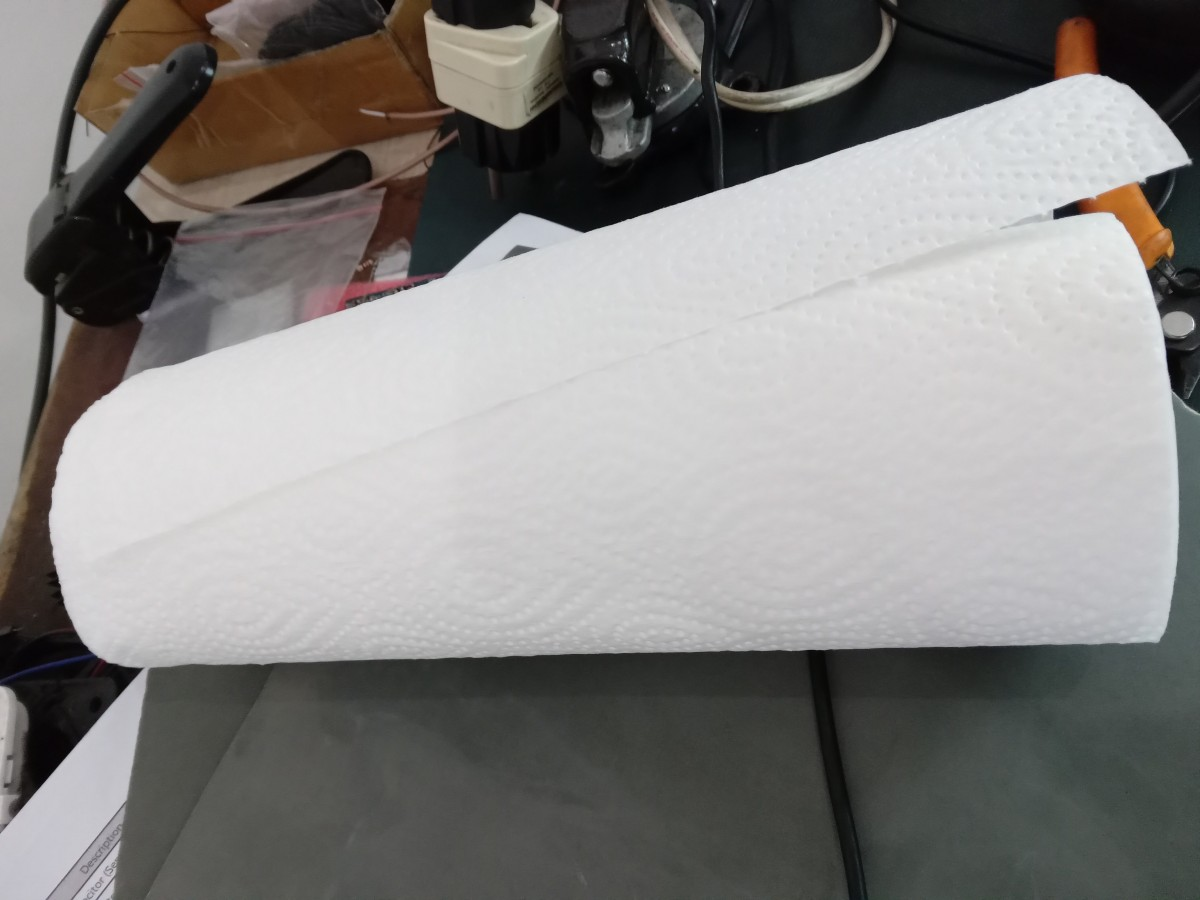
\includegraphics[width=100pt,angle=-90,origin=c]{images/pcbclean1}
		\end{exampleblock}
	\end{frame}

	\begin{frame}
		\begin{exampleblock}{Pensil kayu (membantu menahan posisi komponen QFN/QFP)}
			\centering
			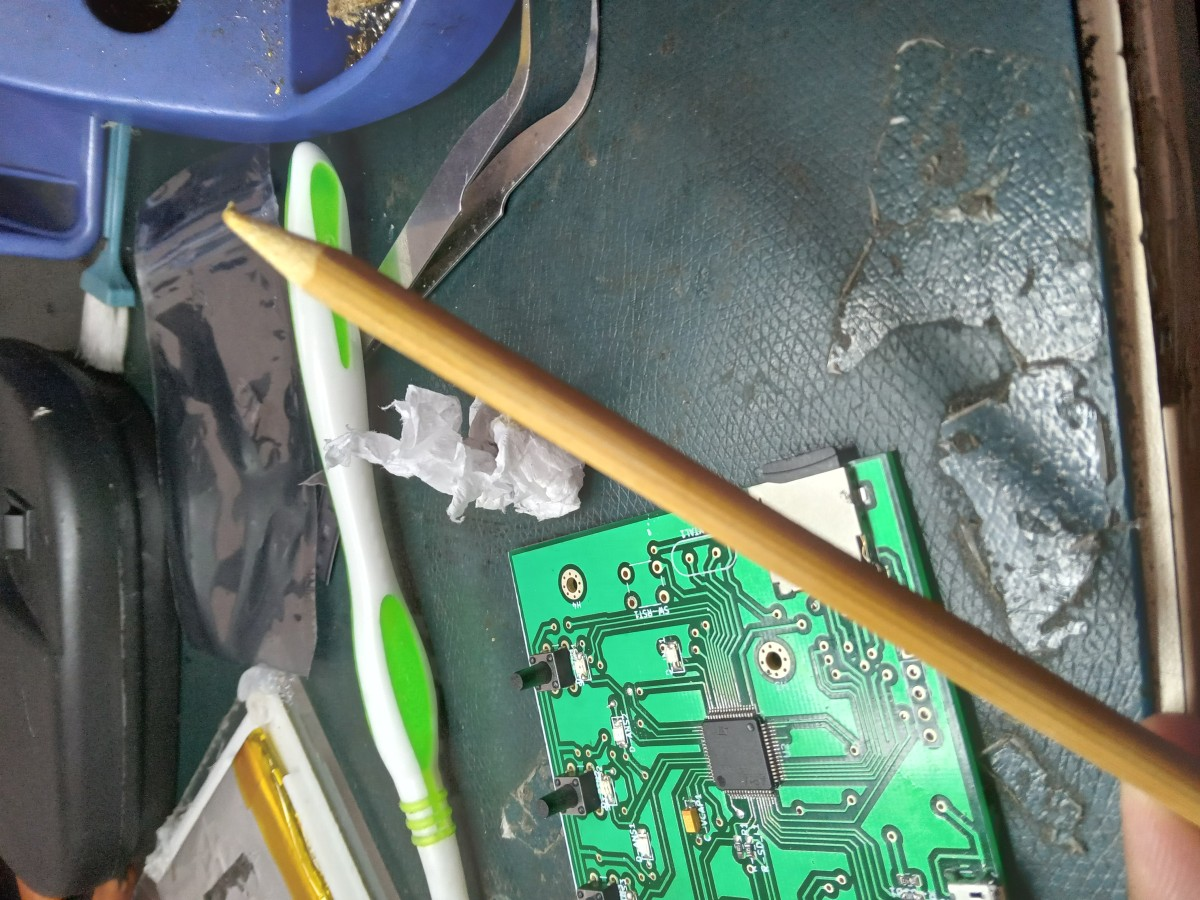
\includegraphics[width=125pt]{images/pensil_kayu}
		\end{exampleblock}

		\begin{exampleblock}{Wire Stripper}
			\centering
			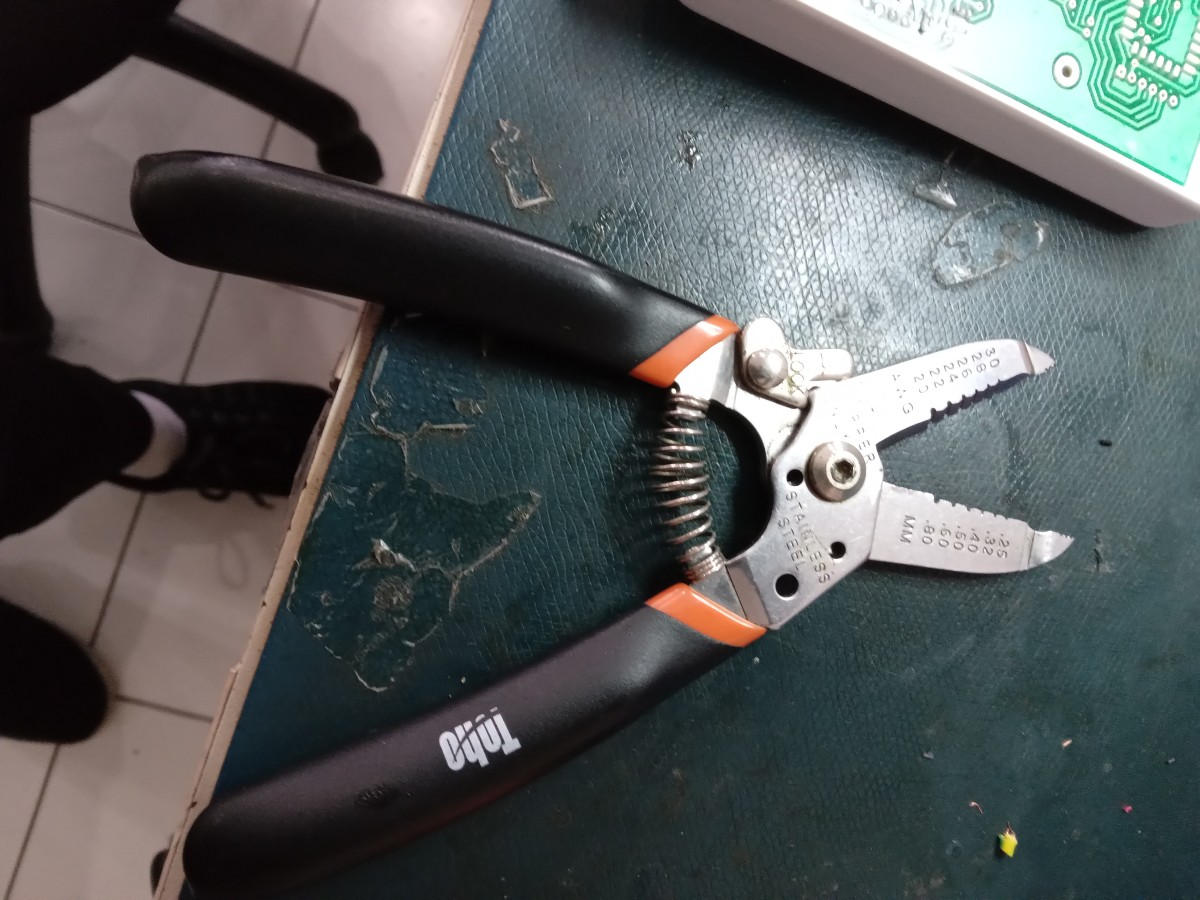
\includegraphics[width=125pt]{images/tang_kabel}
		\end{exampleblock}
	\end{frame}

	\begin{frame}
		\begin{exampleblock}{Osiloskop dan (opsional) Signal Generator}
			\centering
			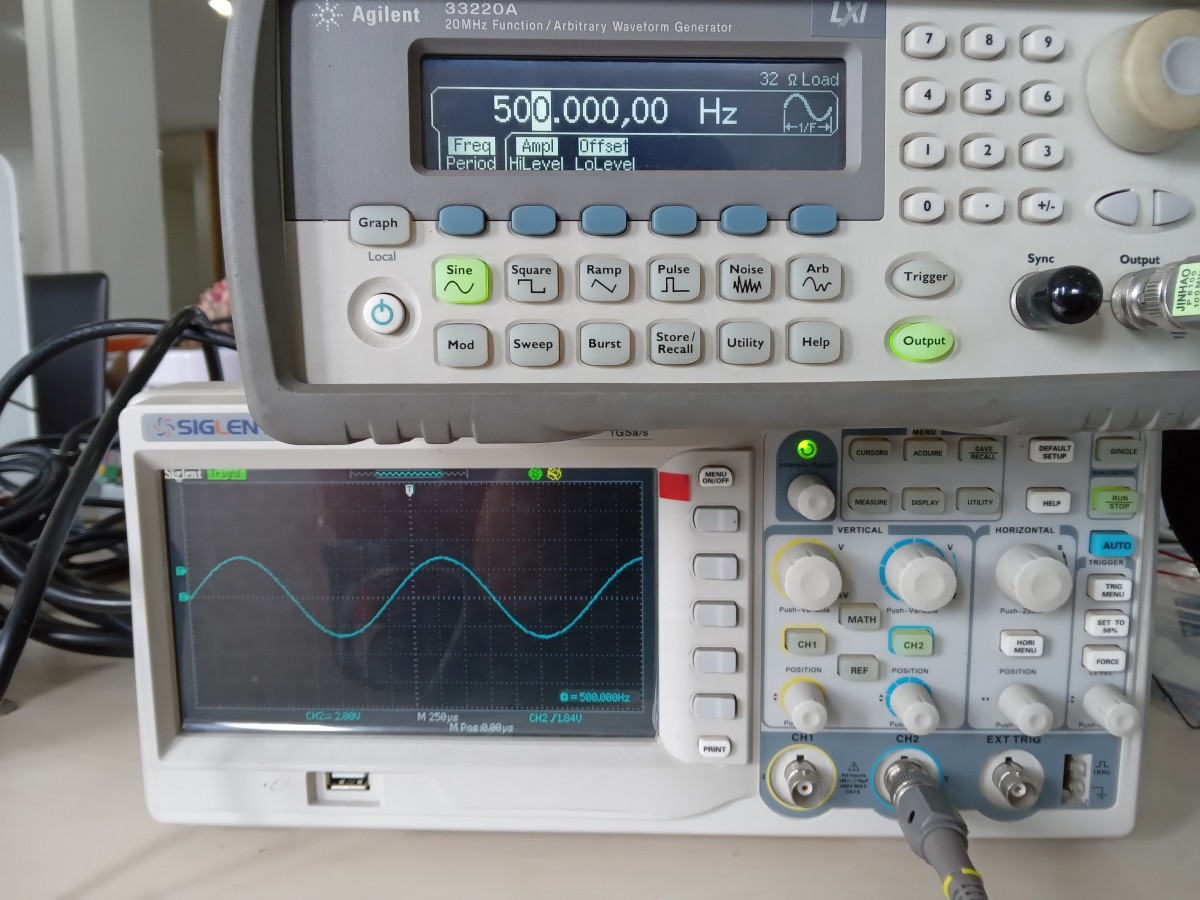
\includegraphics[width=200pt]{images/osi_siggen}
		\end{exampleblock}
	
		\begin{exampleblock}{Catatan}
			\begin{itemize}
				\item Osiloskop dengan sample rate di atas 300kHz (Switching Rate MAX98357A)
				\item Signal Generator mampu untuk Low-Impedance (High Amplitude)
			\end{itemize}
		\end{exampleblock}
	\end{frame}
	
	\subsection{Wishlist}
	
	\begin{frame}
		\begin{exampleblock}{Daftar Rencana Belanja}
			\begin{itemize}
				\item Solder Station Cellkit 936A/936D. Rp. 312,000\\
				\href{https://www.tokopedia.com/archive-dyahgaleryy-1630682557/solder-cellkit-936-analog-ck-936a-limited}{Tokopedia}
				
				\item Mata Solder Cellkit 936 Pisau (K-series). Rp. 25,000\\
				\href{https://www.tokopedia.com/cellkit/mata-solder-cellkit-936-model-pisau-miring-rohs-lead-free}{Tokopedia}
				
				\item IPA 1 Liter. Rp. 45,000\\
				\href{https://www.tokopedia.com/netafarmsurabaya/alkohol-ipa-isopropyl-alcohol-99-kemasan-1-liter}{Tokopedia}
				
				\item Wire Stripper. RP. 30,000\\
				\href{https://www.tokopedia.com/gudangperkakas18/tang-kupas-kabel-tang-potong-kabel-wire-stripper-7-inch-3-in-1}{Tokopedia}
				
				\item Smoke Absorber. \sout{Rp. 423,000} (PO/Not-Ready)\\
				\href{https://www.tokopedia.com/greenmall88/fa-400-solder-iron-smoke-absorber-fume-extractor-soldering-air-blower}{Tokopedia}
			\end{itemize}
		\end{exampleblock}
	\end{frame}

	\begin{frame}
		\begin{exampleblock}{Daftar Pilihan Belanja Osiloskop}
			\begin{itemize}
				\item Hantek DSO5102P 100MHz 2CH. Rp. 4,400,000\\
				\href{https://digiwarestore.com/id/oscilloscopes/digital-storage-oscilloscope-hantek-dso5102p-osiloskop-100mhz-2-ch-641135.html}{Digiware}\\
				\href{https://www.tokopedia.com/digiware/digital-storage-oscilloscope-hantek-dso5102p-osiloskop-100mhz-2-ch}{Tokopedia}
				
				\item Siglent SDS 1072CML 100MHz 2CH. Rp. 6,820,000\\
				\href{https://www.tokopedia.com/tomas123/siglent-sds-1072cml}{Tokopedia}
				
				\item Siglent SDS 1102CML 100MHz 2CH. Rp. 12,450,000\\
				\href{https://www.tokopedia.com/tomas123/siglent-sds-1072cml}{Tokopedia}
				
				\item Siglent SDS 2102X 100MHz 2CH. RP 12,700,000\\
				\href{https://www.tokopedia.com/infinity226/super-phosphor-oscilloscope-siglent-sds2102x}{Tokopedia}
			\end{itemize}
		\end{exampleblock}
	
		\begin{exampleblock}{Daftar Pilihan Belanja Signal/Function Generator (\textbf{Opsional})}
			\begin{itemize}
				\item Feeltech FY6600 High Amplitude. Rp. 2,300,000\\
				\href{https://www.tokopedia.com/digilifeweb/signal-function-generator-feeltech-fy6600-60m-60mhz-dds-fy6600-60m}{Tokopedia}
			\end{itemize}
		\end{exampleblock}
	\end{frame}
	
\end{document}
